\documentclass[12pt]{book}

\usepackage[T2A,L7x]{fontenc}
\usepackage[utf8x]{inputenc}
\usepackage[russian,lithuanian]{babel}
\usepackage[svgnames]{xcolor} % Required to specify font color
\usepackage{textcomp}
\usepackage{hyperref}
\usepackage[shortlabels]{enumitem}
\usepackage{graphicx}
\usepackage{wrapfig}
\usepackage{caption}
\usepackage{nicefrac}
\usepackage{gensymb}

\hypersetup{colorlinks, citecolor=black, filecolor=black, linkcolor=black, urlcolor=black}

\title{25 fotografijos pamokos}
\author{V. P. Mikulinas}
\date{1958}

\renewcommand{\thefigure}{\arabic{figure}}
% \addto\captionslithuanian{\renewcommand{\partname}{Dalis}}
\addto\captionslithuanian{\renewcommand{\chaptername}{Pamoka}}
\addto\captionslithuanian{\renewcommand{\figurename}{pieš.}}
\captionsetup[figure]{labelformat=simple, labelsep=space}

\graphicspath{ {/} }

\begin{document}
	\pagenumbering{gobble}% Remove page numbers (and reset to 1)
	\clearpage
	\thispagestyle{empty}

	\maketitle

	\pagebreak
	\cleardoublepage
	\pagenumbering{arabic}% Arabic page numbers (and reset to 1)
	\chapter*{}
	\section*{Autoriaus žodis}
		Fotografija labai paplito moksle, technikoje, visuomeniniame gyvenime, buityje. Fototgrafija --- tarybinės spaudos pagalbininkas; į laikraščius ir žurnalus dedamos nuotraukos supažindina skaitytojus su Tėvynės gyvenimu, rodo mūsų liaudies darbą, kultūrą, poilsį, nušviečia užsienio gyvenimą. Fotografijų mėgėjų skaičius mūsų šalyje pasiekė kelis milijonus.

		Mūsų pramonė kasmet pagamina milijoną fotoaparatų. Trys tūkstančiai aparatų per dieną. Tai reiškia, kad per metus nauji šimtai tūkstančių tarybinių žmonių papildys fotografų mėgėjų eiles.

		Daugeliui pradedančių domėtis fotografija vėliau ji praverčia kasdieniniame darbe --- mokslinėje ekspedicijoje, gamyklos arba instituto laboratorijoje, įmonės arba kolūkio klube ir t. t.. Kai kurie iš jų, gal būt, virs kvalifikuotais fotografais specialistais. Kai kuriems fotografavimas taps patraukliu kultūringu poilsiuarba saviveikliniu menu, kuris artimas dailininkų kūrybai.

		Fotografijos mėgėjai neperšoks per pradinas jos technikos pakopas. Padėti jiems, kiek tai įmanoma, ir ne tik pačioje pradžioje, --- šios knygos uždavinys.

		``25 fotografijos pamokos''  --- ne vadovėlis, o praktiškas vadovas savarankiškai užsiiminėjantiems nespalvotąja fotografija.

		Pirmojoje knygos dalyje išdėstyta tai, kas labiausiai reikalinga pirmai pažinčiai su fotografija --- nuo to momento, kai pradedantis fotografas pirmąkart ima į rankas aparatą, iki gatavo atspaudo padarymo.

		Antrojoje dalyje detalizuojamos pagrindinės fotografinio proceso stadijos. Ši dalis skirta skaitytojams, jau pažįstantiems fotografijos abėcėlę, mokantiems fotografuoti, ryškinti filmą, spausdinti nuotraukas ir norintiems smulkiau studijuoti fotografavimo techniką.

		Trečiojoje dalyje papasakota, kuriuo būdu galima geriausiai nufotografuoti įvairius objektus. Čia išdėstytas kolektyvinis mūsų šalies ir užsienio fotografų patyrimas. Ši dalis skiriama techniškai pasiruošusiems fotografams mėgėjams.

		Kiekvieną ``pamoką'' nebūtina išmokti vienu prisėdimu: ją galima nagrinėti ir savaitę --- kaip kam išeina.

		Suprantama, kad, norint tapti geru fotografu, negana perskaityti knygą. Ji gali duoti pagrindą savarankiškam darbui, išmokyti taisyklingų veiksmų, apsaugoti nuo klaidų, sužadinti norą tobulintis. Visa kita priklauso nuo fotografo mėgėjo atkaklumo ir daugiausia nuo praktikos.

		\textit{Vertėjo pastaba.} Verčiant knygą į lietuvių kalbą, autorius kai kurias teksto vietas pataisė.
	\part{PAGRINDINĖS FOTOGRAFIJOS ŽINIOS}
	\setcounter{section}{0}
	\chapter{Pažintis su fotografija}
	% \section{}
		\textbf{Fotografinio proceso elementai. --- Fotoaparato konstrukcija. --- Medžiagos fotografijai.}
		\section*{Fotografinio proceso elementai}
			Fotografija taip pavadinta, sujungus graikiškus žodžius \textit{photos} (šviesa) ir \textit{grapho} (rašau), ir, išvertus į lietuvių kalbą, reiškia rašymą šviesa, atvaizdų darymą šviesa.

			Šviesos spinduliai, atšokę nuo kokio nors apšviesto daikto ir praėję pro objektyvą, sudaro fotografinės plokštelės (stiklo) arba filmo šviesai jautriame sluoksnyje nematomą \textit{slaptąjį atvaizdą}, kuris po cheminio apdirbimo pavirsta matomu atvaizdu (sudarytu iš atvirkščių tonų) --- \textit{negatyvu}; iš negatyvo daromas ant šviesai jautraus fotografinio popieriaus atspaudas --- \textit{pozityvas}.

			Tokiu būdu, fotografinei nuotraukai padaryti būtini paeiliui trys etapai:
			\begin{enumerate}[1)]
				\item \textit{fotografavimo procesas}, arba fotografavimas (fotografuojamojo daikto atvaizdo ant fotografinės plošktelės arba filmo padarymas fotoaparatu);
				\item \textit{negatyvinis procesas}, arba ryškinimas (cheminis fotografinės plokštelės arba filmo apdirbimas, siekiant paversti slaptąjį atvaizdą matomu --- negatyvu);
				\item \textit{pozityvinis procesas}, arba spausdinimas (galutinio atspaudo ant fotografinio popieriaus padarymas iš negatyvo).
			\end{enumerate}

			\textbf{Fotografavimas.} Norint fotografuoti, reikia turėti prietaisą, kuriuo būtų galima padaryti šviesinį fotografuojamojo daikto atvaizdą ant šviesai jautraus sluoksnio ir kuris kartu apsaugotų šį sluoksnį nuo pašalinės šviesos. Toks prietaisas yra \textit{fotografijos aparatas}. Pagrindinės jo dalys --- šviesos nepraleidžianti \textit{kamera} ir \textit{objektyvas}. Be šių dalių, fotoaparate yra užraktas, reikiamą laiko tarpą atveriąs šviesai kelią į jautrųjį sluoksnį, ir įtaisas keisti atstumui tarp objektyvo ir kameros užpakalinės sienelės. Šis įtaisas leidžia padaryti ryškų atvaizdą daiktų, esančių vienokiu ar kitokiu atstumu nuo aparato; jame yra matinis stiklas arba kitoks prietaisas ryškumui nustatyti.

			Kad būtų vaizdžiau, visą fotografavimo procesą nagrinėsime, taikydami jį plokšteliniams aparatams (``Fotokor'', ``Moskva 3''). Mėgėjai, turintieji filminius fotoaparatus, teperskaito atidžiai (čia ir toliau), kaip veikia plokštelinis aparatas, kaip apdirbama plokštelė, --- tai padės išsiaiškinti procesus, vykstančius fotografimo ir ryškinimo metu. Darbo filminiais aparatais ypatybes vėliau nagrinėsime smulkiai.

			Prieš fotografavimą aparatas išraukiamas, pastatomas ant stovo --- štatyvo (darant momentinę nuotrauką, aparatą galima laikyti rankose), ir objektyvas nukreipiamas į daiktą, kurį numatoma fotografuoti. Paskui atidaromas objektyvas, kuris projektuoja į matinį stiklą sumažintą ir apverstą šviesinį fotografuojamojo daikto vaizdą. Kad šis atvaizdas būtų aiškiau matomas ir kad nekliudytų krintati iš šonų ir iš užpakalio šviesa, kameros užpakalyje yra stogelis. Aparatas pasukamas taip, kad numatytų fotografuoti daiktų atvaizdas tilptų matiniame stikle. Jeigu daiktų atvaizdai dideli ir netelpa, fotografas su aparatu atsitraukia; jeigu jie per maži ir jei norima padaryti didesnį atvaizdą, aparatas priartinamas prie fotografuojamojo daikto.

			Atvaizdas matiniame stikle, tikriausia, bus neryškus, pasklidas. Tada stumiama priekinė aparato dalis į priekį arba atgal (arba sukamas priekinis objektyvo lęšis) tol, kol atvaizdas tampa visiškai ryškus. Tai vadinama \textit{ryškumo nustatymu}.

			Nustačius ryškumą objektyvas uždaromas, išimamas matinis stiklas, ir į jo vietą įstatoma \textit{kasetė} --- tam tikra plokščia šviesos nepraleidžianti dėžutė su ištraukiamu dangteliu. Į kasetę būda įdėta šviesai jautri \textit{plošktelė}. Dabar, atidarius kasetės dangtelį ir objektyvą, į plokštelę projektuosis tas pats atvaizdas, kuris buvo matomas matiniame stikle.

			Fotografuojant ištraukiamas kasetės dangtelis, o paskui paleidžiamas užraktas ir \textit{eksponuojama}, atseit, leidžiama fotografuojamojo daikto šviesiniam atvaizdui tam tikrą apibrėžtą laiką veikti ploštelę, kad jos jautriame sluoksnyje įvyktų pakitimai, po kurių vėliau bus galima gauti pastovų atvaizdą. Paskui kasetės dangtelis įstumiamas, ir kasetė išimama. Tuo fotografavimo procesas baigiamas.

			Tas laiko tarpas, kurį projektuojamas į plokštelę atvaizdas, vadinamas \textit{išlaikymu}. Šis laikas būna labai įvairus --- nuo tūkstantųjų sekundės dalių iki kelių minučių --- ir nustatomas iš pradžių pagal tam tikras lenteles, o paskui, fotografui įpratus, --- iš akies.

			Nufotografavus kasetė kartu su plokštele nunešama į laboratoriją --- tamsų kambarį, apšviestą tam tikra neaktiniška (neveikiančia plokštelės) šviesa. Jeigu kasetė su plokštele būtų nors akimirką atidaryta paprastoje baltoje šviesoje, šviesai jautrus sluoksnis tuojau pat sugestų (nors akis šio pakitimo ir nepastebės). Dėl to reikia rūpestingai saugoti neišryškintas plošteles nuo dirbtinės ar dienos šviesos.\\

			\textbf{Plokštelės ryškinimas.} Atminkite, kad tamsiai raudonoje laboratorijos šviesoje galima apdirbti plokšteles, kurios vazdinamos ``Izoorto'' (ir filmus ``Ortochrom''). Šių plokštelių apdirbimą aprašysime ir toliau.

			Taigi, laboratorijoje, nekenksmingiausioje raudonoje šviesoje, atidaroma kasetė ir išimama plokštelė. Ant jos paviršiaus nematyti jokio atvaizdo: jis kol kas dar nematomas, slaptas, nors fotografuojant, šviesai paveikus, plokštelės fotografiniame sluoksnyje įvyko šiokių tokių pakitimų.

			Kad slaptasis atvaizdas pasidarytų matomas, plokštelė dedama į lėkštą vonelę, į kurią yra įpilta tam tikro tirpalo --- \textit{ryškalo}. Plokštelė vietomis palaipsniuj tamsėja, ant jos pasirodo įvairaus tamsumo juosvai pilkos spalvos vaizdas. Plokštelės šviesai jautrus sluoksnis pakito tose vietose, kurias fotografuojant veikė šviesa. Kuo stipriau veikė šviesa vienas ar kitas plokštelės vietas, tuo labiau jos pakinta ir, vadinasi, tuo labiau patamsėja ryškale. O nuo tamsiųjų fotografuojamojo daikto dalių atšoka į plokštelę maža šviesos, dėl to šios plokštelės vietos  ryškale beveik nepasikeičia, lieka pieniškai gelsvos.

			Slaptojo atvaizdo vertimas matomu vadinamas \textit{ryškinimu}. Ryškinimą reikia baigti, kai visos atvaizdo detalės išryškėja (tam reikia paprastai nuo 4 iki 7 minučių). Jeigu bus ryškinama per ilgai, plokštelė apsitrauks pilkai, apsidengs vualiu.

			Išryškinta plokštelėskaidriai neprasišviečia, yra gelsvo arba rausvo atspalvio ir lieka jautri šviesai. Kad negatyvas pasidarytų visiškai nejautrus šviesai ir skaidrus, kad iš jo vėliau būtų galima spausdinti ant fotografinio popieriaus, jis, paskalautas vandenyje, paneriamas į kitą tirpalą --- \textit{fiksažą}. Iš fiksažo negatyvas išimamas, kai šviesiosios vietos tampa visiškai skaidrios (fiksavimas trunka 10 -- 15 minučių). Po to negatyvas rūpestingai plaunamas vandenyje ir džiovinamas.

			Kaip jau kalbėta, plokštelę ryškinti reikia nekenksmingoje raudonoje šviesoje. Praėjus kelioms minutėms nuo fiksavimo pradžios, laboratorijoje jau galima įžiebti baltą šviesą --- ji plokštelei nebekenkia.

			Ryškinimas ir fiksavimas kartu vadinami \textit{negatyviniu procesu}. Po šio proceso gauname \textit{negatyvą}, kuriame yra fotografuoto daikto atvaizdas, bet su atvirkščiu šviesių ir tamsių vietų išdėstymu: tamsiosios nufotografuoto daikto vietos čia yra šviesios (net ir skaidrios), o šviesiosios daikto vietos čia tamsios (net ir nepermatomos). Negatyvinis atvaizdas yra tarpinis.\\

			\textbf{Atspaudo ant fotografinio popieriaus darymas.} Galutinis fotografavimo tikslas yra padaryti nufotografuoto daikto teisingų tonų atvaizdą. Tuo tikslu išdžiovintas negatyvas uždedamas ant šviesai jautraus fotografinio popieriaus ir apšviečiamas. Šviesa, praėjusi pro negatyvą, veikia fotografinį popieriaus sluoksnį . Kuo tamsesnės atskiros negatyvo vietos, tuo mažiau šviesos jos praleidžia, ir dėl to po tamsiomis negatyvo vietomis šviesa veikia silpnai, po šviesiomis --- stipriau.

			Fotografijos praktikoje naudojami beveik išimtiniai ryškinamieji fotografiniai popieriai, kuriuose atvaizdas išeina nematomas (slaptas), kaip ir plokštelėje fotografavimo metu. Atvaizdą reikia išryškinti, kad jis pasidarytų matomas --- sudarytas iš tonų, atvirkščių negatyvui, ir atitinkąs fotografuotąjį daiktą. Paskui atspaudas fiksuojamas, plaunamas ir džiovinamas. Šie fotografiniai popieriai apdirbami taip pat kaip ir plokštelės negatyviniame procese, tamsiame kambaryje, bet šviesesnėje --- oranžinėje arba šviesiai raudonoje šviesoje.

			Atspaudas ant fotografinio popieriaus vadinamas \textit{pozityvu}, o jo gavimo iš negatyvo operacijos --- \textit{pozityviniu procesu}.

			Atspaudą ant fotografinio popieriaus galima padaryti ne tik aprašytuoju \textit{kontaktiniu} būdu, kurio atspaudas padaromas tokio pat dydžio kaip ir negatyvas, bet ir \textit{projekciniu} spausdinimo būdu, vadinamuoju \textit{fotografiniu didinimu}. Spausdinant šiuo būdu, padidintas negatyvinis atvaizdas projektuojamas tamsiame kambaryje projekciniu žibintu į šviesai jautrų popierių (panašiai, kaip projektuojamas filmas kine į ekraną).

			Trumpai susipažinę, kaip vyksta pagrindiniai fotografinio proceso etapai, pradėsime nagrinėti smulkiau, praktiškai, kiekvieną iš jų atskirai.

			Ši knyga skirta paprastos juodos-baltos fotografijos procesams. Spalvotosios fotografijos ji neliečia. Daugiasluoksnių spalvotųjų fotografibių medžiagų apdirbimas, ypač spalvotųjų pozityvų darymas ant popieriaus, žymiai sudėtingesnis už atitinkamus juodos-baltos fotografijos procesus. Fotografas mėgėjas gali pereiti prie spalvotosios fotografijos tik po to, kai išmoksta paprasto fotografavimo technikos. O pagal principinę schemą abi fotografijos rūšys yra vienodos.
		\section*{Fotoaparato konstrukcija}
			Susipažinsime iš pradžių, kaip sudarytas fotografijos aparatas, kuriuo padaromas šviesinis (optinis) atvaizdas.
			\subsection*{Pagrindinės fotografijos aparato dalys}
				Žiūrint paskirties ir konstrukcijos, fotografijos aparatai turi vienokius ar kitokius prietaisus, skirtus fotografavimo operacijoms suprastinti, palengvinti ir patikslinti, bet sudaryti jie visi pagal vieną principą. Fotografavimo proceso esmė visada lieka ta pati: objektyvas projektuoja kameroje fotografuojamojo daikto optinį atvaizdą, kuris atsispaudžia ant šviesai jautrios plokštelės arba filmo.

				Šių laikų bendros paskirties fotografijos aparatas sudarytas iš šių pagrindinių dalių: 1) kameros (šviesos nepraleidžiančios dėžtuės); 2) objektyvo (prietaiso optiniam atvaizdui sudaryti); 3) užrakto (mechanizmo, kuriuo šviesinis atvaizdas reikiamą laiko tarpą praleidžiamas į plokštelę arba filmą); 4) mechanizmo ryškumui nustatyti; 5) vaizdo ieškiklio (prietaiso fotoaparatui nutaikyti į fotografuojamąjį objektą).

				Būtinas fotoaparato priedas yra kasetė (arba kitoks prietaisas jautriajai fotografinei medžiagai įdėti).
				\subsubsection*{Kamera}
					Kamera, paprastai kalbant, yra šviesos nepraleidžianti dėžutė, kurios vienoje sienelėje įtvirtintas objektyvas, o priešingoje sienelėje įtaisoma šviesai jautri medžiaga (1 pieš.).
					\begin{figure}[h]
						\centering
						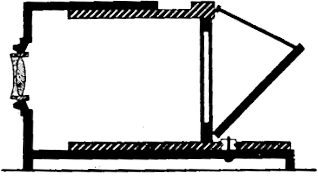
\includegraphics[width=0.8\textwidth]{1-pav}
						\caption{Pirmojo pardavinėjimui skirto fotoaparato pjūvis (Dager, 1839 m. Nuo to laiko kameros schema nepasikeitė)}
						\label{fig:1}
					\end{figure}
					Kamera turi apsaugoti fotografinę plokštelę arba filmą nuo bet kokios pašalinės šviesos. Fotoaparatų kameros arba korpusai būna: a) standūs, dėžutės tipo (``Liubitel''); b) standūs kompaktiški su ištraukiamu objektyvu (FED, ``Zorkij'', ``Kijev''); c) su sustumiamomis dumplėmis, siaurėjančiomis (``Fotokor'', ``Moskva'') arba vienodo skerspjūvio (štatyvinės kameros), panašiomis į armonikos dumples.

					Konstruktoriai stengiasi padaryti tokią kamerą, kuri suglausta užimtų kuo mažiau vietos.
				\subsubsection*{Objektyvas}
					Svarbiausia fotoaparato dalis --- objektyvas. Tai yra optinis prietaisas, projektuojąs į plokštelę arba filmą fotografuojamojo daikto šviesinį atvaizdą.
					\begin{wrapfigure}{r}{0.33\textwidth}
						\centering
						
\includegraphics[width=0.33\textwidth]{2-pav}
						\caption{Pusiau suklijuoto keturių lęšių anastigmato ``Industar'' konstrukcinė schema}
						\label{fig:2}
					\end{wrapfigure}
					Paprastas surenkamas lęšis (didinamasis stiklas) duoda pasklidą, neryškų atvaizdą. Dėl to objektyvai, kurie dabar naudojami fotografijoje, paprastai yra sudaryti iš kelių (nuo trijų iki aštuonių) lęšių, kurių iškilumas arba įdubimas (kreivumo spinduliai) ir stiklo sudėtis tiksliai apskaičiuoti ir išlaikyti gaminant. Gretimi lęšiai atskiriami oro tarpu arba suklijuojami. Tokie tobuli objektyvai vadinami \textit{anastigmatais}; jie duoda aiškų ir ryškų atvaizdą. Visuose mūsų šalyje gaminamuose fotoaparatuose įstatyti anastigmatai (2 pieš.).

					Objektyvas montuojamas įtvare, atitinkančiame kamerą, kuriai jis skirtas. Aparatų su centriniu užraktu objektyvai įmontuoti įtvare, kuris sujungtas su užraktu; mažojo formato aparatų objektyvai --- dvigubame įtvare su sriegiais, kurių dėka objektyvą galima pastumti (sukant) išilgai optinės ašies ir tuo nustatyti atvaizdo ryškumą; štatyvinių kamerų objektyvų įtvarai vadinami normaliais įtvarais.

					Ant objektyvo įtvaro išgraviruota: vienos ar kitos rūšies objektyvo pavadinimas, jo židinio nuotolis ir santykinė anga (šviesos stiprumas), o kai kada ir gaminusio fabriko markė bei eilės numeris. Ten pat arba ant centrinio užrakto įtvaro padaryta diafragmų skalė, o daugumoje šiuolaikinių objektyvų --- ir atstumų skalė bei ryškumo zonos skalė.

					Židinio nuotolis ir santykinė anga yra pagrindiniai objektyvą apibūdinantieji duomenys.\\
				
					\textbf{Židinio nuotolis.} Židinio nuotoliu (pagrindiniu) vadinamas atstumas tarp objektyvo optinio centro ir plošktelės (arba filmo), kai ryškiai nustatytas labai tolimo daikto atvaizdas. Jeigu objektyvas nustatytas taip, kad labai tolimų daiktų (pavyzdžiui, trobesio ir kt., esančių ne arčiau kaip už 100 \textit{m} nuo aparato) atvaizdas matiniame stikle išeina ryškus (tai vadinama ryškumo nustatymu begalybei), tai atsumas tarp objektyvo diafragmos plokštumos ir matinio stiklo yra lygus to objektyvo židinio nuotoliui\footnote{Tai galioja objektyvams, kurių diafragmos plokštuma eina per optinį centrą. Daugumai objektyvų tas atstumas tik apytikriai bus lygus objektyvo židinio nuotoliui. Teleobjektyvams šios taisyklės taikyti negalima.}. Kiekvieno objektyvo židinio nuotolis --- tai tas mažiausias atstumas nuo jo optinio centro iki plokštelės, kuriuo tegalima gauti ryškų atvaizdą. Fotografuojant arčiau esančius daiktus, atstumą tarp objektyvo ir plokštelės tenka padidinti; norint daiktą nufotografuoti natūralaus didumo (neperžengiant aparato plokštelės dydžio ribų), reikėtų dumples ištempti dvigubu objektyvo židinio nuotolio dydžiu --- reikėtų panaudoti \textit{dvigubo ilgio} dumples. Iš mūsų šalyje masiškai gaminamų fotoaparatų tiktai ``Fotokor'' turi dvigubo ilgio dumples; dėl to kitais aparatais negalima fotografuoti labai arti (arčiau kaip už 1,3 -- 1,5 \textit{m}) esančių daiktų, nepanaudojus papildomų prietaisų.

					Židinio nuotolis išreiškiamas centimetrais (arba milimetrais). Nuo jo dydžio priklauso objektyvo šviesos stiprumas ir ryškiai atvaizduojamos erdvės zona, daiktų atvaizdų mastelis ir, be to, kiekvienai objektyvo konstrukcijai --- didžiausias plokštelės arba filmo formatas, kuriuo galima padaryti iki kraštų ryškų atvaizdą.

					Fotografuojant iš to paties taško, objektyvas su trumpu židinio nuotoliu duoda mažo formato atvaizdą smulkiu masteliu, objektyvas su ilgu židinio nuotoliu duoda didelio formato atvaizdą stambiu masteliu. Atvaizdų mastelis yra tiesiog proporcingas židinių nuotoliams.

					Normaliais židinių nuotoliais laikomi: 9 \texttimes 12 \textit{cm} negatyvui --- 13,5 centimetro; 6 \texttimes 9 \textit{cm} negatyvui --- 11 centimetrų; 6 \texttimes 6 cm negatyvui --- 7,5 centimetro; mažojo formato negatyvui (24 \texttimes 36 mm) --- 5 centimetrai.\\

					\textbf{Santykinė anga (geometrinis šviesos stiprumas).} Objektyvo šviesos stiprumu vadinama jo galia apšviesti vienokiu ar kitokiu stiprumu kameroje esančios fotografinės medžiagos šviesai jautrų sluoksnį. Šviesos stiprumo dydžio reikšmė didelė: kuo didesnis objektyvo šviesos stiprumas, tuo mažesnio išlaikymo (plokštelės arba filmo apšvietimo laiko) reikia fotografuojant.

					Suprantama, kad objektyvas su didele anga praleidžia daugiau šviesos negu objektyvas su maža anga. Tačiau absoliutus objektyvo skersmens dydis dar nieko nenuliame. Iš tikrųjų: jeigu palyginsime objektyvą su langu, pro kurį į tamsią patalpą (kamerą) patenka šviesa, tai nesunkiai įsitikinsime, kad bet kuris daiktas (plokštelė arba fimas) bus apšviestas tuo stipriau, kuo didesnis pats langas ir kuo arčiau yra tas daiktas.

					Vadinasi, objektyvo šviesos stiprumas priklauso nuo dviejų dydžių: nuo angos dydžio ir nuo židinio nuotolio. Objektyvo šviesos stiprumas tuo didesnis, kuo didesnė jo anga ir kuo trumpesnis jo židinio nuotolis.

					Šis ryšys išreiškiamas \textit{santykinės angos} dydžiu, kuris yra santykis tarp pilnos objektyvo veikančiosios angos\footnote{Pilna veikiančiąja anga vadinama didžiausia objektyvo anga (įeinamasis vyzdys), pro kurią praeina šviesos spindulių pluoštas; ji paprastai lygi pirmajam lęšiui arba kiek mažesnė už jį (išimtis --- plačiakampiai objektyvai).} skersmens ir jo pagrindinio židinio nuotolio (žinoma, abu dydžiai imami vienodais ilgio vienetais). Pavyzdžiui, angos skersmuo (2 \textit{cm}) sutinka su židinio nuotoliu (8 \textit{cm}) kaip 2 : 8; po suprastinimo (padalijus santykį iš pirmojo nario dydžio) gaunama 1 : 4 --- tai ir yra santykinės angos skaitinė reikšmė.

					Fotoaparato FED objektyvo pilnos angos skersmuo 14,3 \textit{mm}, židinio nuotolis 50 \textit{mm}, o padaliję iš pirmojo nario dydžio (14,3), gausime 1 : 3,5.

					Santykinė anga žymima santykiu tarp vieneto ir skaičiaus, rodančio, kiek kartų to objektyvo pilnos angos skersmuo mažesnis už jo židinio nuotolį.

					Šiuolaikiniuose aparatuose būna objektyvai su santykinėmis angomis 1 : 1,5; 1 : 2; 1 : 2,8; 1 : 3,5; 1 : 4; 1 : 4,5; 1 : 6,3. Kuo didesnis antrasis santykio narys, tuo mažesnė pati santykinė anga. Tai suprantama: santykinės angos skaitinė reikšmė yra trupmena. O kadangi \nicefrac{1}{4} yra mažiau už \nicefrac{1}{2}, tai ir santykinė anga 1 : 4 yra mažesnė už angą 1 : 2.

					Objektyvo anga --- tai skritulys; kaip žinome iš geometrijos, skritulių plotai sutinka kaip jų skersmenų kvadratai. Vadinasi, vieno objektyvo šviesos stiprumas sutinka su kito šviesos stiprumu kaip atitinkamų santykių angų skersmenų kvadratai. Tačiau yra paprastesnis būdas nustatyti, kiek kartų vieno objektyvo šviesos stiprumas didesnis už antrojo: didesnįjį dviejų santykinių angų vardiklį reikia padalyti iš mažesniojo vardiklio ir gautą dalmenį pakelti kvadratu (padauginti patį iš savęs). Pavyzdys: sulyginamas šviesos stiprumas objektyvų, kurių santykinės angos 1 : 4,5 ir 1 : 1,5.
					\[
						(4,5 : 1,5)^{2} = 3^{2} = 9.
					\]

					Vadinasi, antrojo objektyvo šviesos stiprumas yra 9 kartus didesnis už pirmojo, ir, kai anga visa atidaryta, viendomis fotografavimo sąlygomis antrajam objektyvui reikia 9 kartus mažesnio išlaikymo (suapvalinus, pavyzdžiui, \nicefrac{1}{100} sekundės vietoj \nicefrac{1}{10} sekundės).

					\textbf{Diafragma.} Ant objektyvo (apatinėje centrinio užrakto dalyje arba tiesiog ant įtvaro) yra eilė didėjančių skaičių, pavyzdžiui, tokių: 4,5 --- 5,6 --- 8 --- 11 --- 16 --- 22 --- 32 (``Moskva'') arba 3,5 --- 4,5 --- 6,3 --- 9 --- 12,5 --- 18 (FED), kurių pirmasis visada sutampa su objektyvo santykinės angos vardikliu.

					Atidarę centrinį užraktą ir nustatę esančią prie skaitmenų rodyklę-slankiklį ties mažiausiu skaičiumi, pamatysime, kad objektyvo anga atidaryta visa. Jeigu slankiklį stumsime didesnių skaičių link, objektyvo anga palaipsniui mažės ir ties didžiausiu skaičiumi bus mažiausia. Prietaisas objektyvo angai reguliuoti vadianamas \textit{diafragma}, o skaičių eilė --- tai šio prietaiso skalė.

					Šių laikų objektyvuose naudojama vadinamoji irisinė diafragma; ji sudaryta iš lapelių, esančių tarp objektyvo lęšių (maždaug jo optinio centro plokštumoje) ir sudarančių beveik apskritą angą. Susieidami arba prasiskirdami, lapeliai palaipsniui keičia objektyvo veikiančiosios angos dydį (3 pieš.).

					Skaičiai diafragmų skalėje yra objektyvo faktinių (veikiančiųjų) santykių angų vardikliai įvairioms slankiklio padėtims. Jie apskaičiuojami tuo pačiu principu, kaip ir pilna santykinė anga, bet skaitiklis, visada lygus vienetui, patogumo dėlei nežymimas (4 pieš.).

					Diafragma vadinama ir pati reguliuojamoji anga, žymint jos dydį atitinkamu skaitiniu rodikliu (diafragma 5,6) arba išreiškiant jį žodžiais (didelė diafragma, maža diafragma).
					\begin{figure}[h]
						\centering
						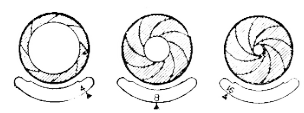
\includegraphics[width=0.8\textwidth]{3-pav}
						\caption{Irisinė diafragma}
						\label{fig:3}
					\end{figure}
					\begin{figure}[h]
						\centering
						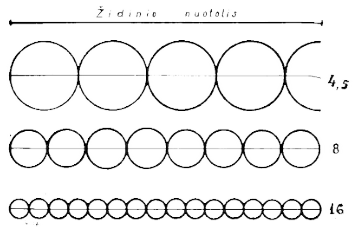
\includegraphics[width=0.8\textwidth]{4-pav}
						\caption{Diafragmos kiekvienos angos dydis žymimas skaičiumi, kuris rodo, kiek kartų angos skersmuo telpa objektyvo židinio nuotolyje}
						\label{fig:4}
					\end{figure}
					Pastaruoju atveju turimas galvoje angos dydis, bet ne skaičius, kuriuo ta anga pažymėta skalėje. Didelė diafragma --- tai didelė anga, bet maži skaičiai (1,5 -- 4,5). Maža diafragma --- tai maža anga, bet dideli skaičiai (11 -- 36). Vidutinė diafragma --- tai 5,6 -- 9\footnote{Diafragmos anga visais atvejais laikoma veikiančioji objektyvo anga. Ji lygi šiek tiek padidintam diafragmos vaizdui, matomam pro priekinį lęšį.}.

					Kad būtų trumpiau, sutarsime toliau (tik šioje knygoje) objektyvo šviesos stiprumo dydį žymėti vien tik pilnosios santykinės angos vardikliu, panašiai kaip žymima diafragmų skalėje.

					Siaurindamas objektyvo praleidžiamų šviesos spindulių pluoštą, diafragmavimas sumažina plokštelės arba filmo apšvietimo laipsnį, ir dėl to jau reikia pailginti išlaikymą fotografuojant. Kuo mažesnė naudojamoji diafragmos anga, tuo ilgesnis turi būti išlaikymas.

					Reikia atminti, kad, pavyzdžiui, diafragmos 4 anga visai ne 2 kartus mažesnė už diafragmos 2 angą, bet 4 kartus, ir dėl to išlaikymo su šia diafragma reikia ne du, bet keturis kartus ilgesnio.
					\begin{figure}[h]
						\centering
						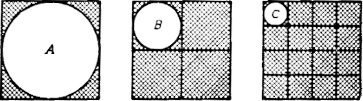
\includegraphics[width=0.8\textwidth]{5-pav}
						\caption{Sumažėjus skritulio skersmeniui 2 kartus, skritulio plotas sumažėja $2^{2}$, atseit, keturis, kartus. Skritulių $A$, $B$ ir $C$ skersmenys sutinka kaip 1 : \nicefrac{1}{2} : \nicefrac{1}{4}, o jų plotai kaip 1 : \nicefrac{1}{4} : \nicefrac{1}{16}}
						\label{fig:5}
					\end{figure}
					Tai paaiškinama tuo, kad diafragmos angos numeruojamos pagal jų skersmenis, o apskritų angų plotai sutinka kaip skersmenų kvadratai. Dėl to, sumažėjus 2 kartus angos skersmeniui, jos plotas sumažėja $2^{2} = 4$ kartus.

					Šį santykį vaizdžiai paaiškina 5 piešinys. Nesunku įsitikinti, kad vidurinio skritulio $B$ skersmuo lygiai du kartus mažesnis už kairiojo skritulio $A$ skersmenį; tuo tarpu jo plotas keturis kartus mažesnis, ir, vadinasi, anga $B$ praleis šviesos 4 kartus mažiau negu anga $A$. Dešiniojo skritulio $C$ skersmuo yra 4 kartus mažesnis už kairiojo skritulio $A$ skersmenį, o jo plotas 16 kartų mažesnis. Tas pats ir su diafragmos angomis.

					Kintamų diafragmų skalė sudaryta taip, kad kiekvienai gretimai diafragmai išlaikymo reikia dukart ilgesnio (jeigu anga sumažinama) arba dukart trumpesnio (jeigu anga padidinama)\footnote{Išimtis daroma tiktai pilnajai angai, kai jos dydis neįeina į standartinę diafragmų eilę.}. Tokiu būdu, sumažinus angą per dvi skalės padalas, išlaikymas paketurgubėja ir t. t.

					Žemiau, 1 lentelėje, parodoma (šiek tiek apvalinti) dafragmų angų ir reikalingų išlaikymų priklausomybė.
					\begin{table}[h]
						\caption{\textbf{Priklausomybė tarp diafragmos ir išlaikymo}}
						\begin{tabular}{c|c|c|c|c|c|c|c|c|c|c|}
							\hline
							Diafragma & $\frac{1,4}{1,5}$ & 2 & 2,5 & 2,8 & 3,5 & 4 & 4,5 & 5,6 & 6,3 & 6 \\ \hline
							Santykinis išlaikymo dydis & 1 & 2 & 3 & 4 & 6 & 8 & 10 & 16 & 20 & 32 \\
							\hline
						\end{tabular}
						\begin{tabular}{c|c|c|c|c|c|c|c|c|c|}
							\hline
							Diafragma & 9 & 11 & 12,5 & 16 & 18 & 22 & 25 & 32 & 36 \\ \hline
							Santykinis išlaikymo dydis & 40 & 64 & 80 & 128 & 160 & 256 & 320 & 512 & 640 \\
							\hline
						\end{tabular}
					\end{table}

					Iš lentelės matyti, kad diafragmai 32 reikia 50 kartų ilgesnio išlaikymo negu diafragmai 4,5 ir maždaug 500 kartų ilgesnio išlaikymo negu pilnai objektyvo angai 1,5. Jeigu objektyvas, kurio šviesos stiprumas 2, diafragmuojamas iki 5,6, tai išlaikymą reikia pailginti 8 kartus (16 : 2).

					Diafragmų (vadinasi, ir išlaikymų) reikšmės yra vienodos bet kuriems objektyvams, nepriklausomai nuo jų konstrukcijos, židinio nuotolio ir pilno šviesos stiprumo. Jeigu dviejuose objektyvuose, iš kurių vieno švieos stiprumas 1,5, kito --- 4,5, nustatysime diafragmą 8, tai fotografuojant abiem atvejais išlaikymo reikia vienodo\footnote{Geometrinio šviesos stiprumo požiūriu.}.

					Kam gi reikalinga išlaikymą ilginanti diafragma? Žinoma, ne tiktai atvaizdui ant plokštelės ar filmo patamsinti, nors objektyvo praleidžiamos šviesos sumažinimas būna naudingas, kai objektas nušviestas skaisčios saulės, negatyvinė medžiaga labai jautri, objektyvo šviesos stiprumas didelis, trumpiausiasis užrakto automatiškai atliekamas išlaikymas per ilgas, ir be diafragmavimo būtų neišviangiamas negatyvo peršvietimas (perlaikymas).

					Pagrindinė diafragmavimo paskirtis yra gauti ryškų atvaizdą, praplečiant vidanamąją ryškiai vaizduojamos erdvės zoną tais atvejais, kai norima viename negatyve nufotografuoti iš karto objektus, esančius įvairiais atstumais nuo aparato (vieni arti, kiti toliau arba labai toli).

					\textit{Apie praskaidrintuosius objektyvus.} Daugumas mūsų šalyje gaminamų fotoobjektyvų yra praskaidrinti, kitaip sakant, juose sumažintas kiekis šviesos, kuri paprastai atšoka ir išsisklaido nuo lęšių paviršių ir dėl to arba nepasiekia plokštelės ar filmo, arba sukuria vualį. Paskaidrinimas padidina atvaizdo kontrastą, maždaug 30\% sumažina išlaikymą. Be to, paskaidrintas objektyvas sumažina aureolių susidarymą, duoda švaresnį atvaizdą, kai fotografuojama prieš šviesą ir fotografuojant objektus su smarkiai atspindinčiais paviršiais (sniegas saulėje, vanduo, stiklas ir pan.). Objektyvai paskaidrėja, aptraukus lęšių poliruotus paviršius, susisiekiančius su oru, mikroskopiškai plonu skaidriu sluoksniu, kuris suteikia jiems violetiškai melsvą atspalvį. Kad būtų galima įsivaizduoti skaidrinančio sluoksnio storį, pažymėsime, kad jis lygus \nicefrac{1}{1000} paprastos filminės juostelės storio.

					Tai ir visos žinios apie objektyvą, reikalingos pradedančiajam fotografui mėgėjui iš pradžių, juo labiau, kad jau gamykloje į kiekvieną fotoaparatą įdedamas trumpiausias objektyvas, ir rinktis jo nebereikia.
				\subsubsection*{Užraktas}
					Fotografinis užraktas --- mechanizmas, kuris atidaro praėjusiems pro objektyvą šviesos spinduliams kelią į plokštelę arba filmą ir po tiksliai nustatomo laiko tarpo uždaro jį. Užraktu daromas trumpas išlaikymas, kuris dabartinėje fotografijoje (pavyzdžiui, fotografuojant greitai judančius objektus) trunka šimtąsias ir tūkstantąsias sekundės dalis.

					Mėgėjiškuose aparatuose pasitaiko dvejopų užraktų: 1) centrinis užraktas, atidarąs ir uždarąs veikiančiąją objektyvo angą (jis įtaisytas mūsų aparatuose, skirtuose plošktelėms ir plačiam filmui); 2) užuolaidinis užraktas, atidengiąs ir uždengiąs negatyvinės medžiagos plokštumą (jis įtaisytas mūsų mažojo formato filminiuose aparatuose).

					\textit{Centrinis užraktas} taip pavadintas pagal savo veikimo principą. Jo dalis, užstojanti šviesą, yra sudaryta iš kelių metalinių ploštelių-sąvarėlių, esančių tarp lęšių. Ši dalis pradeda objektyvo atidarymą ir baigia jo uždarymą veikiančiosios angos centre. Visa plokštelė apšviečiama vienu metu. Šis užraktas, tikslus laikrodinis mechanizmas, įtaisomas žiedu aplink objektyvą ir sujungiamas su objektyvo įtvaru. Mūsų šalyje gaminami centriniai užraktai automatiškai išlaiko atidarytą objektyvą nuo 1 iki \nicefrac{1}{250} sekundės.

					\textit{Užuolaidinis užraktas} taip pavadintas dėl savo šviesą užstojančios detalės --- šviesos nepraleidžiančios \textit{užuolaidėlės}, kuri sudaryta iš dviejų dalių, atskirtų skersiniu plyšiu. Užuolaidėlė padaryta iš gumuotos šilkinės medžiagos arba sudaryta iš siaurų skersinių metalinių juostelių. Užraktas įmontuotas į fotoaparato korpusą. Veikimo metu užuolaidėlė, persivyniodama nuo vieno velenėlio ant kito, pralekia palei patį filmą, kuris pro užuolaidėlės plyšį apšviečiamas palaipsniui nuo vieno krašto iki kito. Tokie užraktai automatiškai atmatuoja išlaikymą nuo 1 iki \nicefrac{1}{1250} sekundės (išlaikymo dydis reguliuojamas, keičiant plyšio plotį ir užuolaidėlės pralėkimo greitį).

					Tokiu būdu, žemutinė mūsų gaminamų užuolaidinių užraktų išlaikymo riba yra 5 kartus mažesnė negu centrinių užraktų. Abiejų tipų užraktais galima laikyti objektyvą atidarytą kiek patinka, laikant nuspaustą užrakto svirtelę (mygtuką).

					Užraktas --- sudėtingiausia fotoaparato dalis; naudotis juo reikia išmokti tobulai, stebint jo veikimą ant matinio stiklo pro atidarytą užpakalinę kameros sienelę arba iš priekio pro objektyvą.

					Kaip pavyzdį išnagrinėsime, kaip veikia centrinis užraktas ``Moment'' (6 pieš.), kuris įtaisomas fotoaparatuose ``Moskva''. Patogiausia jo darbą stebėti ant aparato ``Moskva 3'' matinio stiklo.

					Atidarę aparatą, atlenkiame stogelį, esantį už matinio stiklo. Jeigu dabar nukreipsime objektyvą į apšviestą langą, tai ant matinio stiklo dar nieko nepamatysime, nes užraktas uždarytas. Norint atidaryti užraktą, reikia iš pradžių pasukti žiedą --- išlaikymo reguliatorių taip, kad raidė \textit{\foreignlanguage{russian}{Д}} atsidurtų ties rodykle viršutinėje užrakto dalyje; nuspaudus užrakto svirtelę (arba mygtukinę žarnelę), užraktas atsidaro.

					Jeigu dabar, atleidę svirtelę, nukreipsime objektyvą į langą, tai kameros matinis stiklas nušvis.
					\begin{figure}[h]
						\centering
						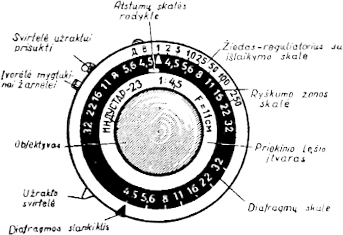
\includegraphics[width=0.8\textwidth]{6-pav}
						\caption{Centrinis užraktas ``Moment''}
						\label{fig:6}
					\end{figure}
					Jeigu vėl paspausime užrakto svirtelę, užraktas užsidarys, ir matinis stiklas vėl pasidarys tamsus. Tokiu būdu, kai reguliatorius nustatytas ties raide \textit{\foreignlanguage{russian}{Д}}, pirmuoju svirtelės paspaudimu užraktas atidaromas, antruoju paspaudimu --- uždaromas. Taip užraktas nustatomas, fotografuojant ilgu išlaikymu (ilgesniu kaip 5 sekundžių).

					Jeigu ties rodykle nustatysime išlaikymo reguliatoriaus raidę \textit{B}, tai atvaizdas ant matinio stiklo bus matomas tik tol, kol užrakto svirtelė laikoma nuspausta. Kai tik jūs atleisite svirtelę, užraktas užsidarys. Taip užraktas nustatomas, fotografuojant trumpesniu išlaikymu (nuo 1 iki 5 sekundžių).

					Pagaliau, jeigu ties rodykle nustatysime kurį nors iš skaitmenų, esančių išlaikymo reguliatoriaus skalėje (nuo \textit{1} iki \textit{250}) ir žyminčių sekundės dalis, o paskui pasuksime užraktą, pasukę jo prisukamąją svirtelę į dešinę iki galo, tai, paspaudus užrakto svirtelę, atvaizdas ant matinio stiklo pasirodys atitinkamą trumpą laiko tarpą ir tuojau pat išnyks. Taip užraktas ``Moment'' nustatomas, fotografuojant 1 -- \nicefrac{1}{250} sekundės išlaikymu (2 lent.).
					\begin{table}[h]
						\caption{\textbf{Priklausomybė tarp diafragmos ir išlaikymo}}
						\begin{tabular}{c|c}
							\hline
							Reguliatoriaus išlaikymas & Naudojimas ir veikimas \\ \hline
							\foreignlanguage{russian}{\foreignlanguage{russian}{Д}} & \textbf{Nustatant ryškumą pagal matinį stiklą. Fotografuojant ilgu išlaikymu (ilgesniu kaip 5 sekundės)} \par Pirmą kartą paspaudus užrakto svirtelę (arba mygtukinę žarnelę), užraktas atsidaro ir lieka atviras tol, kol užrakto svirtelė paspaudžiama pakartotinai \\ \hline
							B & \textbf{Fotografuojant trumpu išlaikymu (nuo 1 iki 5 sekundžių)} \par Užraktas atviras tol, kol laikoma nuspausta užrakto svirtelė. Atleidus svirtelę, užraktas užsidaro. \\ \hline
							1, 2, 5, 10, 25, 50, 100, 250 & \textbf{Fotografuojant užrakto automatiškai reguliuojamu išlaikymu} \par \textit{Nustačius išlaikymo reguliatorių, užraktą reikia prisukti} \par Paspaudus užrakto svirtelę, užraktas atsidaro ir po atitinkamos sekundės dalies (1 sekundė, \nicefrac{1}{2}, \nicefrac{1}{5}, \nicefrac{1}{10}, \nicefrac{1}{25}, \nicefrac{1}{50}, \nicefrac{1}{100} arba \nicefrac{1}{250} sekundės) automatiškai užsidaro \\
						\end{tabular}
					\end{table}

					Fotografuojant nuo štatyvo (tai būtina, kai išlaikymas ilgesnis kaip \nicefrac{1}{20} sekundės), užraktą reikia paleisti, paspaudžiant mygtukinę žarnelę, įsukamą į užrakto mygtuko skylutę.

					Filminių fotoaparatų centriniuose užraktuose nėra padalos \textit{\foreignlanguage{russian}{Д}} (kad pro atvirą objektyvą atsitiktinai nepatektų šviesos į pervniotą filminę juostelę).

					Mažojo formato aparatų užuolaidiniuose užraktuose padalos \textit{\foreignlanguage{russian}{Д}} taip pat nėra (išimtis --- ``Zorkij 3''); senuose aparato FED modeliuose padalą \textit{B} atstoja padala \textit{Z}.

					Kad nesugestų mechanizmai, išlaikymą keisti reikia tiktai tada, kai centrinis užraktas neužvestas ir kai užuolaidinis užraktas prisuktas.

					Kad geriau išsilaikytų bet kurio užrakto spyruoklės, po darbo reikia jo išlaikymo reguliatorių nustatyti ties mažiausiuoju greičiu (kitaip sakant, ties didžiausiu automatiškai reguliuojamu išlaikymu); kai aparatas ilgėliau nenaudojamas, užraktą reikia palikti neužvestą. Nedarbo padėtyje užraktas neturi praleisti į fotografinį jautrųjį sluoksnį jokios šviesos.
				\subsubsection*{Ryškumo nustatymo mechanizmas}
					Turint plokštelinį fotoaparatą su dvigubo ilgio dumplėmis, nesunku vaizdžiai įsitikinti, kad atvaizdo ryškumas priklauso nuo santykio tarp atstumo nuo objektyvo iki fotografuojamojo daikto ir atstumo nuo objektyvo iki matinio stiklo. Fotografuojant labai tolimus daiktus, atstumas tarp objektyvo ir matinio stiklo yra mažiausias --- lygus objektyvo židinio nuotoliui. Kai fotografuojamas labai arti esąs daiktas natūraliu dydžiu, objektyvas turi būti nuo matinio stiklo nutolęs atstumu, lygiu dvigubam židinio nuotoliui. O kai fotografuojamas daiktas, esąs tarp minėtųjų padėčių, dumplės ištempiamos tiek, kad atstumas tarp objektyvo ir matinio stiklo lygus kažkokiam tarpiniam dydžiui tarp vieno ir dviejų židinio nuotolių.

					Tuo būdu, norint gauti ryškų fotografuojamojo daikto atvaizdą, reikia prieš kiekvieną fotografavimą nustatyti objektyvą tam tikru atstumu nuo matinio stiklo, kitaip tariant, \textit{nustatyti ryškumą}.

					Universaliuosiuose plokšteliniuose fotoaparatuose (``Fotokor'') ryškumas nustatomas, atstumiant tolyn nuo matinio stiklo arba pritraukiant arčiau jo objektyvo stovą, kartu ištempiant ar suglaudžiant kameros dumples. Sulankstomuose aparatuose ``Moskva'' ir aparatuose ``Liubitel'' ryškumas nustatomas, keičiant atstumą tarp objektyvo lęšių (sukinėjant priekinį lešį) ir tuo pačiu objektyvo židinio nuotolį. Kinofilminiuose mažojo formato aparatuose ryškumas nustatomas, stumdant išilgai optinės ašies objektyvą, įdėtą į tam tikrą įtvarą ir sklandžiai vaikščiojantį jame sriegiais.

					Kokiu būdu kontroliuojamas ryškumo nustatymas, atseit, kokiu būdu nustatomas kiekvienu atveju reikalingas atstumas tarp objektyvo ir fotografinės plokštelės arba filminės juostelės?\\

					\textbf{Matinis stiklas.} Paprasčiausias ir kartu tiksliausias ryškumo nustatymo kontrolės būdas --- atvaizdo stebėjimas matiniame stikle, kuris fotografuojant pakeičiamas kasete su plokštele, atsiduriančia tiksliai į matinio stiklo plokštumos vietą (plokštelės fotografinis sluoksnis ir matinė stiklo pusė turi būti nukreipti į objektyvą). Visa, ką akys ryškiai mato matiniame stikle, būna ryšku ir ant plokštelės. Šis būdas naudojamas aparate ``Fotokor'', be to, ir aparatuose ``Zenit'' ir ``Liubitel'' (tik čia ryškumas kontroliuojamas pagal matinį skritulėlį veidrodinio vaizdo ieškiklio lęšio centre). Pagal matinį stiklą taip pat parenkamas kadras, kai fotografuojama nuo štatyvo.\\

					\textbf{Atstumų skalė.} Matiniu stiklu naudotis ne visada patogu ir įmanoma dėl fotografavimo sąlygų. Be to, ne kiekvienas fotoaparatas turi matinį stiklą. Dėl to visuose megėjiškuose aparatuose ryškumui nustatyti yra \textit{atstumų skalė}, kurios rodyklė rodo atstumą nuo aparato iki to taško, kurio atvaizdas nustatytas ryškiai.

					Jeigu nustatę kameros matiniame stikle ryškų tolimų trobesių atvaizdą, pažiūrėsime į atstumų skalę, pamatysime, kad jos rodyklė yra ties ženkleliu $\infty$ (šis ženklelis, panašus į paguldytą aštuoniukę, reiškia ``begalybę''). Be šio ženklo, atstumų skalėje dar yra eilė skaitmenų, pavyzdžiui: 1,5 -- 2 -- 3 -- 5 -- 10 (metrų). Jeigu rodyklė yra ties skaitmeniu 5, tai visų daiktų, esančių 5 \textit{m} atstumu nuo aparato, atvaizdai ant matinio stiklo (vadinasi, ir ant plokštelės) bus ryškūs. Ryškumo nustatymas pagal matinį stiklą ir pagal atstumų skalę turi duoti vienodus rezultatus.

					Atstumas nuo aparato iki fotografuojamojo daikto paprastai matuojamas iš akies arba žingsniais. Reikia įprasti matuojant žingsniuoti taip, kad trys žingsniai būtų lygūs dviem metrams (vienas žingsnis --- \nicefrac{2}{3} \textit{m}).

					Paprastesniuose filminiuose fotoaparatuose (``Smena'') atstumų skalė, vadinama taip pat metražine skale, yra vienintelė priemonė ryškumui nustatyti.\\

					\textbf{Tolimatis.} Geriausias tikslaus ryškumo nustatymo būdas --- naudoti perimtą iš artilerijos prietaisų \textit{tolimatį}, optiniu būdu nustatantį atstumą nuo fotoaparato iki fotografuojamojo daikto. Mechaniškai sujungus tolimatį su objektyvu, gauta pusiau automatinė ryškumo nustatymo kontrolė. Kai tolimačio langelyje dvigubas kokio nors daikto atvaizdo kontūras susilieja į vieną, tai reiškia, kad ir objektyvas ryškiai nustatytas į tą patį daiktą.

					Optinį tolimatį turi aparatai ``Moskva 2'', FED, ``Zorkij'', ``Kijev''.
				\subsubsection*{Vaizdo ieškiklis}
					Vaizdo ieškiklis skirtas fotoaparatui nutaikyti į fotografuojamus daiktus: jis rodo, kas išeis nuotraukoje tais atvejais, kai fotografuojamojo kadro\footnote{Kadru šiuo atveju laiko ta erdvės dalis, kurios atvaizdas telpa fotografinėje plokštelėje arba filminėje juostoje.} ribos nenustatomos pagal matinį stiklą (kameroje nėra matinio stiklo arba, jeigu jis ir yra, fotografuojama ne nuo štatyvo).

					Vaizdo ieškiklių būna rėminių (tiesioginių) ir optinių, kurie skirstomi į tiesioginius ir veidrodinius.
					\begin{figure}[!h]
						\centering
						\begin{minipage}[t]{0.4\textwidth}
							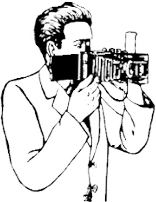
\includegraphics[width=\textwidth]{7-pav}
							\caption{Fotografavimas sulankstomu fotoaparatu}
							\label{fig:7}
						\end{minipage}
						\hfill
						\begin{minipage}[t]{0.4\textwidth}
							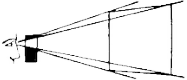
\includegraphics[width=\textwidth]{8-pav}
							\caption{Rėminio vaizdo ieškiklio veikimo principas}
							\label{fig:8}
						\end{minipage}
					\end{figure}

					Patogiausi yra tiesioginiai vaizdo ieškikliai, kuriuos naudojant aparatas laikomas akių lygyje (7 pieš.), ir todėl perspektyva, atvaizduojama ieškiklyje, yra labiau įprasta žiūrovui.

					Rėminis vaizdo ieškiklis (ikonometras) sudarytas iš dviejų rėmelių: mažo ir didelio (negatyvo dydžio); rėmeliai yra nutolę vienas nuo kito atstumu, lygiu objektyvo židinio nuotoliui. Primerkęs vieną akį, antrąja fotografas žiūri pro abu rėmelius. Artindamas akį prie mažojo rėmelio, fotografas randa tokią padėtį, kai visos keturios mažojo rėmelio kraštinės sutampa su visomis keturiomis didžiojo rėmelio kraštinėmis, ir paskui nutaiko aparatą į fotografuojamąjį daiktą. Tuomet visa, kas matyti pro abu rėmelius, išeis ir negatyve (8 pieš.). Rėminis vaizdo ieškiklis rodo vaizdą natūralaus didumo ir yra labai patogus vizuoti. Toks vaizdo ieškiklis yra aparate ``Fotokor'' ir (kaip antrasis vaizdo ieškiklis) aparate ``Liubitel'' (viršutinėje sulankstomojoje šachtoje).

					Atlenkiamas tiesioginis optinis vaizdo ieškiklis sudarytas iš dviejų stačiakampių lęšių: sklaidomojo ir renkamojo (okuliaro), įdėtų į atlenkiamus įtvarus-rėmelius; toks ieškiklis yra fotoaparatuose ``Moskva''.

					Toks pat vaizdo ieškiklis, bet standžios konstrukcijos, su lęšiais, įdėtais į bendrą įtvarą (okuliaras apskritas), montuojamas mažojo formato aparatuose. Laikant fotoaparatą akių lygyje (9 pieš.), pro vaizdo ieškiklio okuliarą matomas labai sumažintas, bet aiškus ir šviesus fotografuojamojo daikto vaizdas.
					\begin{figure}[h]
						\centering
						\begin{minipage}[t]{0.4\textwidth}
							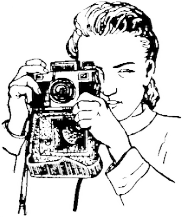
\includegraphics[width=\textwidth]{9-pav}
							\caption{Fotografavimas mažojo formato fotoaparatu}
							\label{fig:9}
						\end{minipage}
						\hfill
						\begin{minipage}[t]{0.4\textwidth}
							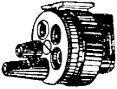
\includegraphics[width=0.4\textwidth]{10-pav}
							\caption{Universalus optinis vaizdo ieškiklis mažojo formato aparatams}
							\label{fig:10}
						\end{minipage}
					\end{figure}

					Mažojo formato fotoaparatams gaminamas pridedamas universalusis optinis vaizdo ieškiklis (10 pieš.), kurio detalė yra pasukamas skridinys su penkiais įvairiais okuliariniais lęšiais.
					Pasukus skridinį, vienas iš lęšių įsijungia į optinę vaizdo ieškiklio sistemą, ir ieškiklis rodo tikslų kadrą atitinkamam vienam iš penkių keičiamųjų objektyvų (kurių židinio nuotolis 2,8; 3,5; 5; 8,5 arba 13,5 \textit{cm}).
					\begin{wrapfigure}{r}{0.25\textwidth}
						\centering
						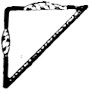
\includegraphics[width=0.25\textwidth]{11-pav}
						\caption{Veidrodinio vaizdo ieškiklio pjūvis}
						\label{fig:11}
					\end{wrapfigure}

					Veidrodinis optinis vaizdo ieškiklis (11 pieš.) sudarytas iš dviejų renkamųjų lęšių, iš kurių vienas, mažesnis, įstatytas vertikaliai, o kitas, didesnis, --- horizontaliai viršutinėje vaizdo ieškiklio dalyje; tarp jų 45\degree kampu į abu lęšius įtvirtintas veidrodis, nuo kurio atšoka į viršų spinduliai, praėję pro mažąjį lęšį.
					Dėl to didysis lęšis sudaro veidrodiškai apverstą fotografuojamojo daikto atvaizdą. Veidrodinis vaizdo ieškiklis blogas tuo, kad į jį žiūrėti reikia iš viršaus, dėl to, naudojant veidrodinį ieškiklį, fotoaparatą tenka laikyti fotgrafo juosmens lygyje (12 pieš.), ir nuotrauka atvaizduoja perspektyvą kiek kitaip, negu paprastai mato mūsų akis. Didelis veidrodinis vaizdo ieškiklis įtaisytas fotoaparato ``Liubitel'' korpuso viršutinėje dalyje.
					\begin{figure}[h]
						\centering
						\begin{minipage}[t]{0.4\textwidth}
							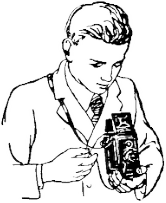
\includegraphics[width=0.4\textwidth]{12-pav}
							\caption{Vizavimas pro dviejų objektyvų fotoaparato veidrodinį vaizdo ieškiklį}
							\label{fig:12}
						\end{minipage}
						\hfill
						\begin{minipage}[t]{0.4\textwidth}
							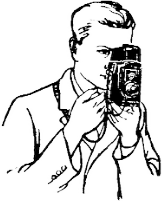
\includegraphics[width=0.4\textwidth]{13-pav}
							\caption{Vizavimas pro dviejų objektyvų fotoaparato rėminį vaizdo ieškiklį}
							\label{fig:13}
						\end{minipage}
					\end{figure}
				\subsubsection*{Kasetės}
					Kasetė yra šviesos nepraleidžiąs metalinis dėklas, į kurį įdėta negatyvinė medžiaga įstatoma į fotoapartą, o po fotografavimo išimama iš jo.

					Plokštelės kasetė --- plokščia, sudaryta iš korpuso ir ištraukiamo dangtelio, į ją telpa viena fotografinė plokštelė. Fotografuojant ji įstatoma į fotoaparatą vietoj matinio stiklo. Aparato ``Fotokor'' kasetės įstumiamos į kameros užpakalinės sienelės išėmas. Aparato ``Moskva 3'' kasetės priglaudžiamos prie kameros užpakalinės sienelės ir pritvirtinamos skląsteliu. Didelių štatyvinių fotokamerų kasetės --- medinės, dvigubos (po vieną plokštelę iš abiejų pusių).

					Mažojo formato fotoaparato filminės juostelės kasetė yra cilindrinės formos, sudaryta iš ritės, korpuso ir dangtelio (FED, ``Zorkij'', ``Zenit'', ``Smena'') arba iš ritės ir dviejų cilindrinių korpuso dalių (``Kijev'', ``Zorkij 3''). Į kasetę telpa 165 \textit{cm} ilgio filminė juostelė --- joje galima padaryti 36 nuotraukas.

					Nuo atsarginių kasečių skaičiaus priklauso, kiek nuotraukų fotografas gali padaryti, negrįždamas į tamsią patalpą.

					Fotoaparatai, skirti plačiam ritiniam filmui, kasečių neturi, filmo juostelė į juos įdedama tiesiog, suvyniota į ritę kartu su šviesos nepraleidžiančiu apsauginiu popieriumi.
			\subsection*{Medžiagos fotografijai}
				\textbf{ŠVIESAI JAUTRIOS MEDŽIAGOS}\\
				Yra medžiagų, kurios nesikeičia patamsyje, bet tuojau pat pasikeičia, kai jas pasiekia šviesa. Šią savybę (jautrumą šviesai), ir labai ryškią, turi sidabro halogenidai, metalinio sidabro junginiai su vienu iš halogenų --- bromu, chloru ar jodu. Sidabro bromidas, chloridas ir jodidas yra fotografinių sluoksnių jautrusis pagrindas.

				Fotografijai naudojami šviesai jautrūs sluoksniai (arba fotografiniai sluoksniai) --- tai plona želatininė plėvelė, kurioje yra labai daug smulkučių šviesai jautraus sidabro halogenido dalelių (mikrokristalų). Kadangi šis sluoksnis pats yra labai plonas ir nestiprus, jis užliejamas ant stipraus pagrindo: ant siklo (fotografinės plokštelės), ant celiulioido (fotofilmas ir kinofilmas), ant popieriaus (fotografinis popierius).

				Pagal paskirtį šviesai jautrios medžiagos (arba fotografinės medžiagos) skirstomos į negatyvines, naudojamas fotografavimui, ir pozityvines --- atspaudams gaminti.

				\subsubsection*{Negatyvinės medžiagos}
					Fotografinės plokštelės ir filmai (filmo juostelės) skiriasi jautrumu šviesai, kontrastiškumu, spektriniu jautrumu; šios jų savybės pažymimos ant pakelių.

					\textit{Jautrumas šviesai} (jautrumas baltos šviesos poveikiui) --- svarbiausia negatyvinių medžiagų savybė: kuo jautrumas didesnis, tuo trumpesnio išlaikymo reikia fotografuojant. Mūsų šalyje gaminamų fotografinių medžiagų jautrumas šviesai išreiškiamas GOST\footnote{\begin{otherlanguage*}{russian}ГОСТ --- Государственный общесоюзный стандарт\end{otherlanguage*} (Valstybininis visasąjunginis standartas).} vienetais. GOST vienetų skaičius tiesiog proporcingas jautrumui: dukart didesnis skaičius reiškia, kad ir jautrumas šviesai dukart didesnis\footnote{Vokiškų fotografinių medžiagų jautrumas šviesai žymimas DIN laipsniais (DIN --- Deutche Industrie Norm). Pagal šią sistemą jautrumas du kartus padidėja (arba sumažėja) kas 3\degree: filmas, kurio jautrumas 18\degree DIN, yra dukart jautresnis už 15\degree DIN filmą (į vardiklį 10, esantį po skaitine laipsnių reikšme, dėmesio nekreipkite --- nuo jo jautrumas šviesai nepriklauso).}.

					Pradedančiajam fotografui mėgėjui, fotografuojančiam palankiomis šviesos sąlygomis, geriau naudoti mažo jautrumo (11 -- 16 GOST vienetų), nedidelio (22 -- 32 GOST vien.) ir vidutinio jautrumo (45 -- 65 GOST vien.) negatyvines medžiagas. Didelio jautrumo fotografinės medžiagos imamos tik tais atvejais, kai šviesos sąlygos nepalankios: kai ūkanotą dieną fotografuojami greitai judantieji objektai, kai daromos momentinės nuotraukos patalpoje. Bet pradedančiajam tokias nuotraukas daryti dar ne laikas.

					Negatyvinės medžiagos \textit{kontrastiškumas} --- tai jos savybė duoti atvaizdus su didesniu ar mažesniu skirtumu tarp tamsiausių ir šviesiausių vietų. Pagal kontrastiškumo laipsnį negatyvinės medžiagos būna labai minkštos (mažai kontrastiškos), normalios, kontrastiškos, labai kontrastiškos, kontrastiškiausios.

					Negatyvinės medžiagos kontrastiškumą reikia derinti su fotografuojamo objekto kontrastiškumu ir jo apšvietimo pobūdžiu. Į minkštus fotografinius sluoksnius fotografuojami kontrastiški ir kontrastiškai (saulės arba dirbtinės šviesos) apšviesti objektai, į kontrastiškus fotografinius sluoksnius --- monotoniški objektai arba, kad ir ne monotoniški, bet fotografuojami ūkanotą dieną; į normalius --- vidutinio kontrastiškumo ir vidutiniškai apšviesti objektai.

					Paprastai fotografinis sidabro bromido sluoksnis jautrus tiktai violetiniams, mėlyniems ir žydriems spinduliams (neskaitant nematomų ultravioletinių); kiti spinduliai (žali, geltoni, oranžiniai, raudoni) jo neveikia. O mūsų akis, atvirkščiai, geltonus spindulius priima kaip šviesiausius, o mėlynus --- kaip tamsiausius. Kai taip nesutampa akies ir fotografinio sluoksnio spalvinis jautrumas, nuotrauka, padaryta ant paprastos (nejautrios spalvoms) plokštelės, atrodo mums tarytum neteisingai perteikianti spalvoto objekto šviesumą: tamsiai mėlynas dangus išeina baltas, o skaisčiai geltoni rugiai --- tamsiai pilki. Siekiant praplėsti fotografinio sluoksnio jautrumo ribas, jis gaminimo metu papildomai įjautrinamas (sensibilizuojamas) kitiems spinduliams. Toks papildomas fotografinio sluoksnio jautrumas spalvoms ir vadinamas \textit{spektriniu jautrumu}\footnote{Fotografinio sluoksnio spektrinio jautrumo (jautrumo spalvoms) nereikia painioti su jo bendruoju jautrumu šviesai, išreiškiamu GOST vienetais; fotofilmas gali būti vidutinio jautrumo šviesai (45 GOST vien.) ir būti plačiai spektriškai įjautrintas (panchromatinis) arba atvirkščiai, būti itin jautrus šviesai (130 GOST vien.) ir su mažu spektriniu jautrumu (ortochromatinis).}.

					Dabar visos negatyvinės medžiagos (išskyrus specialiąsias) gaminamos jau turinčios vienokį ar kitokį spektrinį jautrumą, kuris atsispindi jų pavadinime. Ortochromatinės ir izoortochromatinės medžiagos papildomai įjautrintos (nekalbant jau apie violetinius, mėlynus ir žydrus spindulius) žaliems ir geltoniems spinduliams; izochromatinės medžiagos jautrios taip pat ir oranžiniams spinduliams. Panchromatinės ir izopanchromatinės medžiagos, sensibilizuotos dar ir raudoniems spinduliams, yra jautrios visiems matomiems spinduliams ir dėl to gali atvaizduoti fotografuojamojo objekto šviesumą natūraliausiai.

					Fotografui mėgėjui tenka atsižvelgti į vienos ar kitos negatyvinės medžiagos apdirbimo sąlygas. Nesensibilizuotas medžiagas galima šviesiai raudonoje laboratorinėje šviesoje dėti į kasetes ir ryškinimo indelį, ryškinti vonelėje, o ortochromatines ir izoortochromatines medžiagas --- tamsiai raudonoje šviesoje. Kitoms medžiagoms (izochromatinėms, panchromatinėms, izopanchromatinėms) turi įtakos net tamsiai raudona šviesa, ir dėl to jas dėti į kasetes ir apdirbti reikia visiškame patamsyje, o tai pradedančiajam fotografui mėgėjui sudaro didelių ir net neįveikiamų sunkumų (negalima akimis stebėti plokštelių ryškinimosi eigos). Dėl to pradedančiajam fotografui mėgėjui patariame naudoti izoortochromatines plokšteles ir ortochromatinius filmus, kurie visiškai tinka įvairiausioms nuotraukoms.

					\textit{Fotografinės plokštelės} --- stiklinės plokštelės, aptrauktos iš vienos pusės šviesai jautriu sluoksniu, būna standartinių formatų, priderintų prie aparatų matmenų (nuo 6 \texttimes 9 iki 50 \texttimes 60 \textit{cm}). Jos pardavinėjamos dėžutėse po 12 plokštelių (iki formato 13 \texttimes 18 \textit{cm}).

					Fotofilmai gaminami tokie.

					\textit{Plokštieji fotofilmai} --- formatiniai (nuo 6 \texttimes 9 iki 30 \texttimes 40 \textit{cm}) celiulioido lapai su fotografiniu sluoksniu iš vienos pusės. Parduodami pakeliais po 12 lapų.

					\textit{Ritiniai fotofilmai:}
					\begin{enumerate}
						\item Platusis ritinis filmas yra celiulioidinė 6 \textit{cm} pločio ir 81,5 \textit{cm} ilgio juosta, aptraukta šviesai jautriu sluoksniu ir suvyniota į ritę kartu su ilga šviesos nepraleidžiančia popieriaus juosta, kuri apsaugo filmą nuo pašalinės šviesos. Išorinėje popieriaus juostos pusėje dviem eilėmis atspausdinti eilės numeriai, atitinkantieji atskiras nuotraukas: viena eilė skirta aštuonioms 6 \texttimes 9 \textit{cm} formato nuotraukoms, kita --- dvylikai 6 \texttimes 6 \textit{cm} formato nuotraukų. Ritė su filmu ir šviesos nepraleidžiančia popieriaus juosta įdedama tiesiog į fotoaparatą.
						\item Fotofilmas mažojo formato aparatams --- tai normalus kinofilmas, atseit, celiulioidinė 35 \textit{mm} pločio juostelė, aptraukta fotografiniu sluoksniu ir su skylutėmis palei kraštus (perforuota): skylutės skirtos filmą traukiančiam kameros mechanizmui. Filmo juostelės ilgis --- 165 \textit{cm}, joje telpa 36 negatyvai, kurių formatas --- 24 \texttimes 36 \textit{mm}.
					\end{enumerate}

					Fotografinių plokštelių pranašumas: galima ryškinti atskirai kiekvieną negatyvą. Jų trūkumai: palyginti griozdiškos ir sunkios; reikia tamsaus kambario, įdedant į kasetes. Plokštieji filmai naudojami kaip plokštelės, bet yra lengvesni už jas ir užima mažiau vietos.

					Ritinių filmų pranašumai: vieną kartą įdėjus į aparatą, galima daryti daug nuotraukų; jie lengvi ir portatyvūs; ritę pakeisti galima šviesoje. Jų naudojimas nepatogus tuo, kad reikia ryškinti visą juostą iš karto, bet iš dalies tai gali tapti gera savybe, nes paspartina apdirbimą.

					Pagal naudojamą negatyvinę medžiagą fotografiniai aparatai skirstomi į plokštelinius, plačiafilmius ir siaurafilmius (mažojo formato).

					Fotografinės plokšteles ir plokščiuosius filmus reikia įsigyti pagal savo fotoaparato formatą. Platusis 6 \textit{cm} ritinis filmas tinka visiems mūsų šalyje gaminamiems filminiams aparatams. Kinofilmas vienodai tinka visiems mažojo formato fotoaparatams.
				\subsubsection*{Pozityvinės medžiagos}
					Fotografinis popierius skirstomas į dvi kategorijas: 1) matomai spausdinamą popierių, arba dieninį (pavyzdžiui, aristotipinis), kuris po kontaktinio spausdinimo dienos šviesoje, praėjus palyginti neilgam laiko trapui, duoda matomą atvaizdą, užfiksuojamą viraže-fiksaže; 2) ryškinamą popierių, kuris, spausdinant dirbtinėje šviesoje, per keletą sekundžių duoda slaptą atvaizdą, ryškinamą taip pat kaip plokštelėse ir filmuose.

					Popierių su matomu atvaizdu jau seniai iš pramoninės ir pofesionalios praktikos visiškai išstūmė ryškinamasis popierius: šis leidžia dirbti nepalyginamai greičiau, geriau išsilaiko, tinka didinimui. Dieninio fotografinio popieriaus jau beveik nebevartoja ir mėgėjai, ir mes nebeminėsime jo nei čia, nei toliau.

					\textit{Ryškinamasis popierius} priklausomai nuo to, kurio sidabro halogenido daugiausia įeina į šviesai jautraus sluoksnio sudėtį, skirstomas į sidabro bromido (``Unibrom'' ir ``Bromoserebriannaja''), sidabro chlorido-bromido (``Kontabrom'' ir ``Bromportret''), sidabro chlorido (``Fotokont''), sidabro chlorido-bromido-jodido (``Jodoserebriannaja'') popierių.

					Fotografinis popierius yra žymiai mažiau jautrus šviesai negu negatyvinės medžiagos. Jis jautrus tiktai violetiniams, mėlyniems ir žydriems spinduliams, dėl to jį galima ryškinti geltonoje, oranžinėje, šviesiai raudonoje laboratorinio žibinto šviesoje (kokioje šviesoje galima dirbti --- nurodyta ant pakelių), o taip pat žalioje šviesoje.

					Fotografinis popierius būna įvairaus kontrastiškumo laipsnio. Kontrastiškumas pažymimas ir numeriu: Nr. 1 --- minkštas (mažo kontrastiškumo) popierius, Nr. 2 ir Nr. 3 --- normalus, Nr. 4 ir Nr. 5 --- kontrastiškas, Nr. 6 --- ypatingai kontrastiškas, Nr. 7 --- kontrastiškiausias. Kuo didesnis numeris, tuo didesnis popieriaus kontrastiškumas.

					Fotografinio popieriaus formatai --- nuo 6 \texttimes 6 iki 50 \texttimes 60 \textit{cm}. Popierius parduodamas pakeliuose po 10 ir 20 lapų arba dėžutėse po 100 lapų.

				\textbf{CHEMINĖS MEDŽIAGOS}\\
				Plokštelių, filmų, fotografinio popieriaus cheminiam-fotografiniam apdirbimui naudojami daugiausia du tirpalai: ryškalas, paverčiąs slaptąjį atvaizdą matomu, ir fiksažas, padarąs fotografinį atvaizdą atsparų šviesai. Antrojoje knygos dalyje kiekivenas fotografas mėgėjas išmoks savarankiškai sudarinėti šiuos tirpalus iš pagrindinių cheminių medžiagų, bet iš pradžių patogiau naudotis gatavais fotochemikalų mišiniais, kurie parduodami sausi stikliniuose arba kartoniniuose vamzdeliuose, dėžutėse arba indeliuose --- juos belieka tik ištirpdyti vandenyje.\\

				\textbf{Ryškalai.} Gatavas sausas ryškalas yra kelių cheminių medžiagų miltelių mišinys, perskirtas į dvi nelygias dalis: mažoji dalis --- tai pati ryškinančioji medžiaga, didžioji --- tai kiti reikalingi chemikalai. Etiketėje nurodoma: 1) ryškalo pavadinimas (pagal sudėtį), pavyzdžiui, metolo-hidrochinono, paraaminofenolo; 2) charakteristika --- normalus, smulkiagrūdis; 3) paskirtis (pagal fotografinės medžiagos rūšį) --- plokštelėms ir fotografiniam popieriui, filmui FED; 4) vandens tūris tirpdymui.

				Reikia skirti dvi gatavų preparatų grupes.

				Normalieji arba universalieji ryškalai, kurie dirba sparčiai, naudojami tiktai ploštelėms, plokščiafilmiams ir fotografiniam popieriui ryškinti vonelėse.

				Lėtai veikiantieji (arba smulkiagrūdžiai) ryškalai naudojami tiktai ritiniams filmams (mažojo formato kinofilmui ir plačiajam ritiniam filmui) ryškinti indeliuose. Ryškinti plokštelėms vonelėse, kai ryškinimasis stebimas tiesiog, šie ryškalai nepatogūs (nes lėtai veikia), o fotografiniam popieriui visiškai netinka.

				\textbf{Fiksažai.} Sausą fiksažą galima pirkti paprastą arba rūgštų (rūgšti fiksažo druska). Abiem atvejais fiksuojanti medžiaga yra natrio tiosulfatas (hiposulfitas); į rūgštų fiksažą įeina papildomų medžiagų. Tirpdymui reikalingo vandens tūris nurodomas etiketėse.

				Jeigu įsigyta tik natrio tiosulfato, tai darbinis paprasto fiksažo tirpalas pagaminamas, ištirpdant 1 dalį bevandenio tiosulfato (baltų miltelių) 6 dalyse vandens arba 1 dalį kristalinio tiosulfato (nemažų bespalvių skaidrių kristalų) 4 dalyse vandens (pagal svorį).

				Nors galima išsiversti su paprastu fiksažu, vis dėlto verčiau naudoti rūgštųjį, ypač kinofilmui; jo tirpalas ilgiau išsilaiko nesugedęs.

				Laikykite sausą fiksažą atskirai nuo šviesai jautrių medžiagų ir kitų chemikalų.\\

				Patariama, kai galima, pastoviai vartoti tas pačias negatyvinių ir pozityvinių medžiagų rūšis, tuos pačius ryškalus, kad būtų geriau pažįstamos jų savybės, įgundama kaip reikiant dirbti su jais.

				Šviesai jautrias medžiagas reikia panaudoti (išryškinti), dar nepasibaigus garantiniam tinkamumo laikui, kuris nurodomas ant pakelių bei dėžučių (metai ir mėnuo).
	\chapter{Fotografijos prietaisai}
		\textbf{Mūsų šalyje gaminami fotografiniai aparatai. Fotografijos reikmenys. - Fotografo mėgėjo laboratorija}
		\section*{Mūsų šalyje gaminami fotografiniai aparatai}
			Mūsų Tėvynės pramonė masiškai gamina daug naujausių fotografinių aparatų tipų, panaudodama paskutinius optinės technikos pasiekimus.

			Šios pamokos didžioji dalis skiriama tarybinių fotoaparatų aprašymui, nes norima padėti kiekvienam skaitytojui pasirinkti tinkamiausią aparatą.

			Mes dėstysime tokia tvarka:
			\begin{enumerate}
				\item plokšteliniai fotoaparatai (``Fotokor'', ``Moskva 3'', štatyvinės kameros);
				\item plačiafilmiai fotoaparatai (``Liubitel'', ``Moskva 2'');
				\item kinofilminiai mažojo formato fotoaparatai (FED, ``Zorkij'', ``Kijev'', ``Zenit'', ``Smena'').
			\end{enumerate}
		\subsection*{PLOKŠTELINIAI FOTOAPARATAI}
			Konstrukcinė plokštelinių fotoaparatų ypatybė - matinis stiklas užpakalinėje kameros sienelėje, pagal kurį akimis nustatomas atvaizdo ryškumas; atvaizdas matiniame stikle būna apverstas, bet tiksliai tokios pat išvaizdos, tokio pat dydžio ir ryškumo, koks jis bus negatyve.

			Galimybė spręsti pagal matinį stiklą apie būsimą atvaizdą yra geras dalykas; netogu tiktai, kad po kiekvienos nuotraukos reikia keisti kasetę.

			Plokšteliniai fotoaparatai yra patogūs techninėmis, grupinėms ir kitoms nuotraukoms, kurioms padaryti nereikia didelio operatyvumo. Šie aparatai labiausiai tinka kaip vaizdinė priemonė, mokantis fotografavimo procesų.
		\subsection*{\textit{``Fotokor'' --- plokštelinis 9 \texttimes 12 cm aparatas}}
			``Fotokor'' (14 pieš.) buvo pirmasis masiškai mūsų šalyje gaminamas fotografinis aparatas. Nuo 1941 metų jis nebegaminamas, bet naudojama aparatų ``Fotokor'' daug.
			\begin{figure}[h]
				\centering
				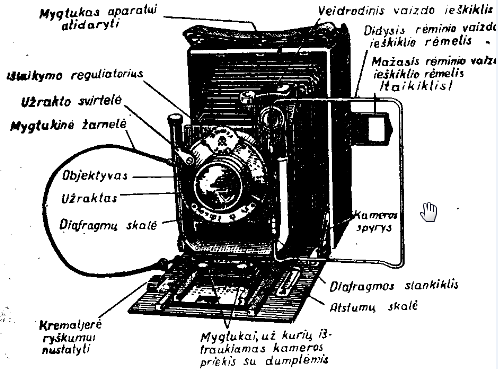
\includegraphics[width=0.8\textwidth]{14-pav}
				\caption{Aparatas ``Fotokor''}
				\label{fig:14}
			\end{figure} 
			Tai skatina mus pradėti apžvalgą kaip tik nuo jo, juo labiau, kad ``Fotokor'' priklauso vadinamųjų universaliųjų fotoaparatų tipui --- fotoaparatų, naudojamų įvairiems darbams.

			``Fotokor'' - sulankstomasis fotoaparatas su matiniu stiklu ir atlenkiama priekine sienele, kuria slankioja objektyvo stovas. Siaurėjančias kameros dumples galima ištempti dvigubai (palyginus su objektyvo židinio nuotoliu). Dumplių ilgis leidžia fotografuoti mažus daiktus iš labai arti (apie 25 \textit{cm}) stambiu masteliu ir net natūralaus didumo, o taip pat naudoti fotoaparatą kaip sudėtinę didinamojo prietaiso dalį. Objektyvą galima pastumti aukštyn ir žemyn, dešinėn ir kairėn, o tai labai svarbu architektūrinei nuotraukai. Joks kitas mėgėjiškas mūsų šalyje gaminamas aparatas šių savybių neturi.

			``Fotokor'' turi keturių lęšių anastigmatą ``Ortagoz'', kurio šviesos stiprumas --- 4,5, o židinio nuotolis --- 13,5 \textit{cm}. Silpna aparato vieta --- jo automatiškai užsivedąs centrinis užraktas \foreignlanguage{russian}{ГОМЗ}, kurio nereikia prieš fotografuojant užvesti ir kuris visada paruoštas fotografavimui, bet automatiškai atlieka tiktai trejopą išlaikymą: \nicefrac{1}{25}, \nicefrac{1}{50} ir \nicefrac{1}{100} sekundės, ir tai, iš vienos pusės, susiaurina greitai judančių daiktų fotografavimo galimybes, o iš kitos --- neduoda fotografui ilgo išlaikymo (iki 1 sekundės), kokio reikia fotografuojant patalpose.

			Fotografuojant aparatu ``Fotokor'', reikia laikytis šių nurodymų:

			\textit{Fotoaparato atidarymas.}
			\begin{enumerate}
				\item Paspausti mygtuką korpuso viršuje --- priekinė aparato sienelė atsidarys.
				\item Atlenkti priekinę aparato sienelę į apačią iki galo --- spyriai turi įsisprengti.
				\item Ištraukti iki galo aparato objektyvo stovą su dumplėmis ir objektyvu (būtinai paėmus už tam skirtų mygtukų).
			\end{enumerate}

			\textit{Fotoaparato uždarymas.}
			\begin{enumerate}
				\item Suspaudus mygtukus, skirtus ištraukti, įstumti aparato objektyvo stovą su dumplėmis į korpusą iki galo. Įdėti mygtukinę žarnelę.
				\item Abu spyrius, laikančius atlenktąją aparato sienelę, paspausti į vidų --- atlenkta sienelė lengvai pakils į viršų.
				\item Galutinai užtrenkti atelnkiamąją sienelę.
			\end{enumerate}

			Aparato ``Fotokor'' užraktas veikia taip.

			Nustačius išlaikymo reguliatorių ties raide \textit{\foreignlanguage{russian}{Д}}\footnote{\textit{\foreignlanguage{russian}{Д}} --- pirmoji raidė rusiško pavadinimo: \begin{otherlanguage*}{russian}Длительная выдержка\end{otherlanguage*} --- ilgas išlaikymas.}, po pirmo mygtukinės žarnelės paspaudimo užraktas atsidaro ir lieka atviras iki antro žarnelės paspaudimo.

			Nustačius ties raide \foreignlanguage{russian}{К}\footnote{\foreignlanguage{russian}{К} --- atitinkamai: \begin{otherlanguage*}{russian}Короткая выдержка\end{otherlanguage*} --- trumpas išlaikymas.}, užraktas atidarytas tol, kol spaudžiamas mygtukas.

			Kai reguliatorius nustatytas ties 25, 50 arba 100, paspaudus mygtukinę žarnelę, užraktas atsidaro tik akimirkai (atseit, \nicefrac{1}{25}, \nicefrac{1}{50} arba \nicefrac{1}{100} sekundės) ir vėl užsidaro. Užvesti užrakto nereikia.

			Ryškumas nustatomas, sukant kremaljerę --- tada objektyvo stovas slenka į priekį ir dumplės išsitempia. Atstumų skalė turi padalas nuo 1,5 \textit{m}.

			Aparatas turi du vaizdo ieškiklius: rėminį ir mažąjį optinį veidrodinį.

			Aparato ``Fotokor'' viengubos kasetės įstumiamos į kameros užpakalinės sienelės išėmas.
		\subsection*{\textit{``Moskva 3'' --- plokštelinis 6,5 \texttimes 9 cm aparatas}}
			``Moskva 3'' (15 pieš.) taip pat yra sulankstomas fotoaparatas su matiniu stiklu, atlenkiama priekine sienele ir siaurėjančiomis dumplėmis. Nuo ką tik aprašyto fotoaparato ``Fotokor'' aparatas ``Moskva 3'' skiriasi štai kuo:
			\begin{enumerate}[1)]
				\item turi tik viengubai ištempiamas dumples, dėl to fotografuoti galima ne iš arčiau kaip 1,5 \textit{m}, ir aparatas netinka nei reprodukcijai, nei mažiems daiktams fotografuoti stambiu masteliu, nei naudoti kartu su didinamuoju prieaparačiu;
				\item jo paskaidrinto keturių lęšių anastigmato ``Industar 23'' šviesos stiprumas --- 4,5, o židinio nuotolis --- 11 \textit{cm}; objektyvo negalima sumdyti nei į šonus, nei į apačią ar viršų;
				\item turi tobulesnį prisukamąjį užraktą ``Moment'', kuris daro aštuoneriopą išlaikymą: 1 sekundė, \nicefrac{1}{2}, \nicefrac{1}{5}, \nicefrac{1}{10}, \nicefrac{1}{25}, \nicefrac{1}{50}, \nicefrac{1}{100} ir \nicefrac{1}{250} sekundės (jis smulkiai aprašytas pirmojoje pamokoje, žr. 6 pieš.);
				\item paspaudus mygtuką aparatui atidaryti, priekinė fotoaparato sienelė, veikiama spyruoklių, atsilenkia į apačią ir kartu mechaniškai svirčių sistemos dėka išlenda ir įsitvirtina priekinis stovas su objektyvu ir dumplėmis; taip aparatas greitai paruošiamas fotografuoti;
				\item ryškumas nustatomas ne ištempiant dumples, bet sukant priekinį objektyvo lęšį: jo įtvare yra ryškumo zonos skalė;
				\begin{figure}[h]
					\centering
					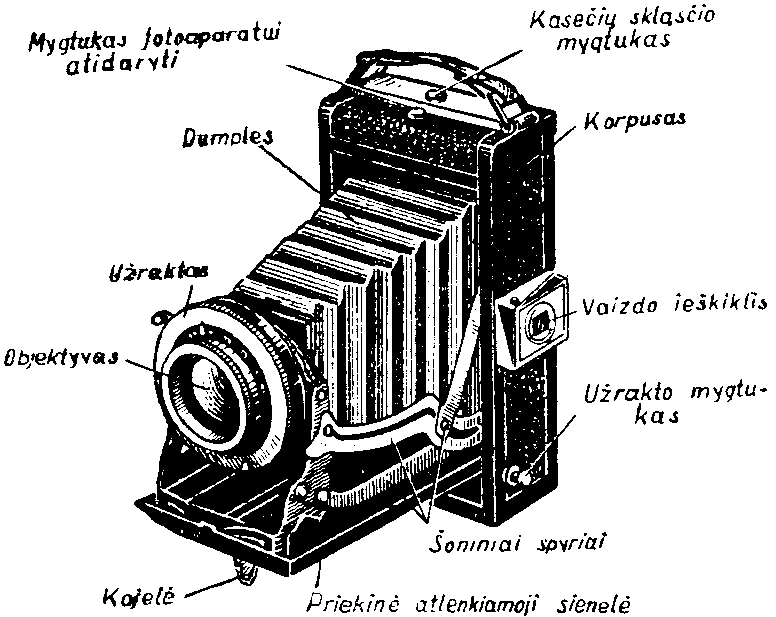
\includegraphics[width=0.8\textwidth]{15-pav}
					\caption{Fotoaparatas ``Moskva 3''}
					\label{fig:15}
				\end{figure}
				\item vaizdo ieškiklis --- tiesioginis optinis: kasetės ne įstumiamos į išėmas, bet priglaudžiamos prie kameros, o tai yra žymiai patogiau.
			\end{enumerate}

			Sulankstyto aparato dydis: 140 \texttimes 90 \texttimes 55 \textit{mm}; svoris --- 720 \textit{g}.

			Prie aparato pridedamos 6 viengubos kasetės.
		\subsection*{\textit{Štatyvinės 13 \texttimes 18 cm ir 18 \texttimes 24 cm kameros}}
			\textit{Štatyvinėmis} fotokameromis (16 pieš.) vadinami palyginti griozdiški suglaudžiami mediniai fotoaparatai su vienodo skerspjūvio dumplėmis ir matiniu stiklu. Šiais aparatais negalima fotografuoti iš rankų, juos būtina pastatyti ant tvirto štatyvo (arba kitokio stovo). Jie yra profesinio tipo fotokameros ir skirti darbams, kuriems reikia stabilaus aparato, didelio negatyvų formato, labai ištempiamų dumplių, įvairiai palenkiamo matinio stiklo, pakeičiamų objektyvų.
			\begin{figure}[h]
				\centering
				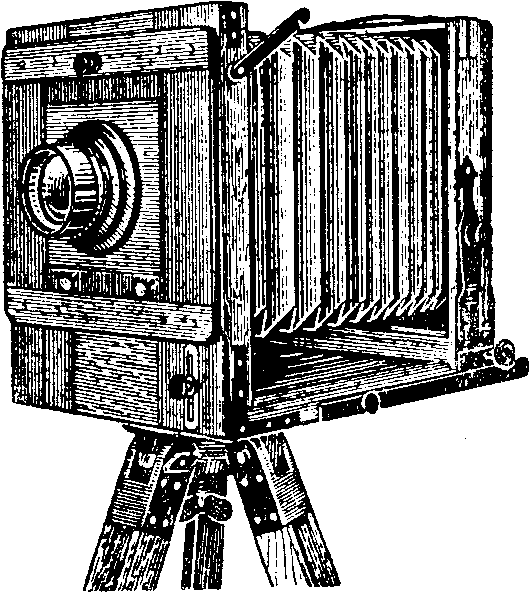
\includegraphics[width=0.8\textwidth]{16-pav}
				\caption{Štatyvinė fotokamera}
				\label{fig:16}
			\end{figure}
			Šios kameros skirtos fotografuoti nuolatinėje patalpoje (portretams, grupėms), išvažiavus (architektūrai, gamtovaizdžiams), daryti mokslinio tyrimo nuotraukoms bei techninėms nuotraukoms laboratorijose ir cechuose, reprodukuoti.

			Kamerų dumplės ištempiamos dvigubai.

			Ryškumas nustatomas kremaljere, kuri stumdo užpakalinę (kasetinę) kameros dalį, kai tuo tarpu priekinė (objektyvinė) dalis nejuda.

			Galima pakeisti objektyvą (kartu su objektyvo lenta).

			Galima ne tik pastumti objektyvą į šonus arba aukštyn bei žemyn, bet ir pakreipti kasetinę dalį, pasukant aplink vertikaliąją ir horizontaliąją ašį.

			Mažoji, 13 \texttimes 18 \textit{cm}, kamera turi keturių lęšių anastigmatą ``Industar 51'', kurio šviesos stiprumas --- 4,5, o židinio nuotolis --- 21 \textit{cm}. Šios kameros dydis: 400 \texttimes 310 \texttimes 220 \textit{mm}; svoris (su priedais) --- 11 \textit{kg}.

			Kita, 18 \texttimes 24 \textit{cm}, kamera turi objektyvą ``Industar 13'', kurio šviesos stiprumas --- 4,5 ir židinio nuotolis --- 30 \textit{cm}. Šios kameros dydis: 500 \texttimes 360 \texttimes 260 \textit{mm}; svoris (su priedais) --- 14 \textit{kg}.

			Fotokameros neturi nei vaizdo ieškiklio, nei užrakto (išlaikymas atliekamas ranka nuimant ir vėl užmaunant ant objektyvo dangtelį).

			Prie kamerų pridedama po tris dvigubas pusiau užuolaidines kasetes, brezentinis dėklas, tvirtas sulankstomas medinis štatyvas su makštimi.

			Su dėklais į kasetes galima įdėti mažesnių formatų plokšteles.

			Štatyvinės fotokameros, kasetės ir plokštelės joms yra sunkios, užima daug vietos; didelių formatų plokštelės brangios. Fotografai mėgėjai šių kamerų nenaudoja. Vis dėlto mes aprašėme jas, manydami, kad kai kuriems skaitytojams vėliau bedirbant, gal būt, teks su jomis susidurti.

			Be to, dideliame, gerai aprūpintame fotografijos būrelyje, kuriam vadovauja patyręs fotografas, štatyvinė fotokamera gali būti sėkmingai naudojama gilesniam fotografijos studijavimui.
		\subsection*{PLAČIAFILMIAI FOTOAPARATAI}
			Konstrukcinė filminių fotoaparatų savybė yra mechanizmas negatyvinėms medžiagoms įdėti. Viršutinėje ir apatinėje korpuso dalyje yra patalpos dviem ritėms. Ritė su filmu į aparatą įdedama baltoje šviesoje. Darant vieną po kitos nuotraukas, filmas rankenėle, esančia kameros šone, vis pavyniojamas nuo tiekiančiosios ritės ant priimančiosios, kad prieš objektyvą kiekvieną kartą atsidurtų neeksponuotas filmo ruožas.

			Besikeičiantiems kadrų numeriams stebėti yra mažas apskritas langelis aklinoje užpakalinėje kameros sienelėje, apsaugotas raudonu šviesos filtru. Išfotografavus visą ritę, ji išimama iš kameros taip pat baltoje šviesoje, o tiekiančioji ritė, iš kurios filmas išsivyniojo, perkeliama į priimančiosios vietą.
		\subsection*{\textit{``Liubitel'' --- filminis 6 \texttimes 6 cm aparatas}}
			Plačiafilmis dviejų objektyvų fotoaparatas ``Liubitel'' (17 pieš.), į kurį įdedamas filmas dvylikai nuotraukų, yra dėžutės pavidalo; priekinėje sienelėje įtaisyti vienas virš kito du objektyvai, sujungti įtvariniais išoriniais krumpliaračiais. Apatinis objektyvas yra fotografuojamasis, o viršutinis (paprastesnsi) yra didelio veidrodinio vaizdo ieškiklio priekinis lęšis (18 pieš.). Nustatant ryškumą, sukamas apatinis krumpliaratis, ir kartu išilgai savų optinių ašių juda ir fotografuojamasis objektyvas, ir viršutinis objektyvas.
			\begin{figure}[h]
				\centering
				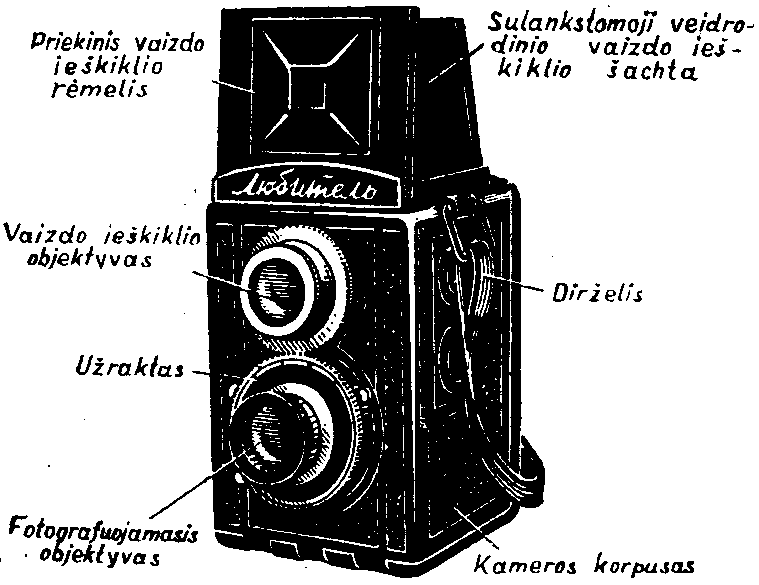
\includegraphics[width=0.8\textwidth]{17-pav}
				\caption{Fotoaparatas ``Liubitel''}
				\label{fig:17}
			\end{figure}

			Tokiu būdu pagal matinę centrinę vaizdo ieškiklio viršutinio horizontalaus lęšio dalį akimis nustatomas ryškumas.

			Kai fotografuojamasis objektyvas diafragmuojamas iki reikiamo laipsnio, pilna viršutinio objektyvo anga (2,8) visada duoda kuo šviesiausią atvaizdą, tuo palengvindama tiksliai vizuoti ir nustatyti ryškumą net iki užrakto paleidimo momento.

			Aparato ``Liubitel'' veidrodinis vaizdo ieškiklis ypač patogus daryti portretinėms nuotraukoms ir fotografuoti scenoms su vaikais. Nors jame matomas atvaizdas neapverstas aukštyn kojomis, kaip paprastai būna matiniame stikle, bet jis veidrodiškai apsuktas (atseit, kairioji ir dešinioji fotografuojamojo objekto pusės sukeistos). Tai neturi reikšmės, fotografuojant daugumą daugiau ar mažiau statiškų objektų, bet nepatogu sportinėms nuotraukoms, nes judąs objektas pasirodo vaizdo ieškiklyje ne iš tos pusės, iš kurios jis faktiškai juda ir iš kur jo nesąmoningai laukia fotografas. Dėl to tokias nuotraukas reikia daryti, naudojant rėminį vaizdo ieškiklį, kurio rėmeliai įjungti į priekinę ir užpakalinę kameros viršutinės sulankstomosios šachtos sienelę.
			\begin{wrapfigure}{l}{0.33\textwidth}
				\centering
				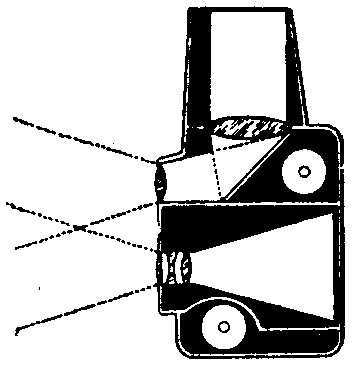
\includegraphics[width=0.33\textwidth]{18-pav}
				\caption{Fotoaparato ``Liubitel'' schema}
				\label{fig:18}
			\end{wrapfigure}

			Kad nepasitaikytų nufotografuoti du kartus ant to paties fotofilmo ruožo, reikia tuojau pat po kiekvienos nuotraukos pervynioti filmą.

			Aparato ``Liubitel'' fotografuojamasis objektyvas --- trijų lęšių anastigmatas ``T-22'', kurio šviesos stiprumas --- 4,5, o židinio nuotolis --- 7,5 \textit{cm}. Centrinis užraktas automatiškai atlieka penkeriopą išlaikymą: \nicefrac{1}{10}, \nicefrac{1}{25}, \nicefrac{1}{50}, \nicefrac{1}{100} ir \nicefrac{1}{200} sekundės.

			Mažiausias atstumas iki fotografuojamojo objekto --- 1,3 \textit{m}.

			Kameros dydis: 135 \texttimes 90 \texttimes 90 \textit{mm}; svoris --- apie 600 \textit{g}.

			Fotoaparato naudojimas nesudėtingas, aparatas skirtas pradedantiems fotografams mėgėjams.

			Dabar jau nebegaminamas fotoaparatas \textit{``Komsomolec''} yra supaprastintas, lyginant su aparatu ``Liubitel'', modelis. Jo veidrodinio vaizdo ieškiklio priekinis lęšis nejudamas, dėl to vaizdo ieškiklis naudojamas tik aparatui nutaikyti į objektą, o ryškumas nustatomas tiktai pagal atstumų skalę. Jo objektyvo šviesos stiprumas beveik du kartus mažesnis (6,3) kaip aparato ``Liubitel''. Užraktas automatiškai atlieka tiktai trejopą akimirkinį išlaikymą: \nicefrac{1}{25}, \nicefrac{1}{50} ir \nicefrac{1}{100} sekundės, dėl to juo ne taip patogu tiek fotografuoti greitai judančius objektus, tiek ir fotografuoti patalpose.
		\subsection*{\textit{``Moskva 2'' --- 6 \texttimes 9 cm filminis aparatas}}
			Sulankstomas plačiakampis fotoaparatas ``Moskva 2'' (19 pieš.) ant vieno filmo padaro 8 nuotraukas. Jo konstrukcija ir išorė panašios į plokštelinio fotoaparato ``Moskva 3'', aprašyto aukščiau, bet jo korpusas kiek ilgesnis ir su nuožambiais kampais.

			Kairėje kameros pusėje pritaisytas tolimatis, sujungtas su objektyvu.
			\begin{figure}[h]
				\centering
				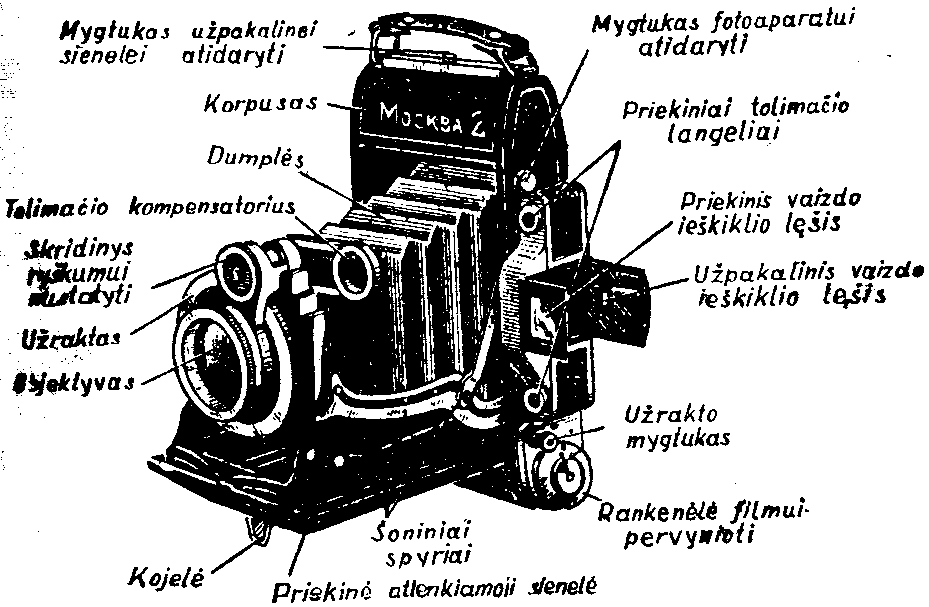
\includegraphics[width=0.8\textwidth]{19-pav}
				\caption{Fotoaparatas ``Moskva 2''}
				\label{fig:19}
			\end{figure}
			Besukant skridinį, esantį virš užrakto, kartu veikiamas tolimačio kompensatorius ir priekinis objektyvo lęšis, kuris pasisukdamas reguliuoja ryškumą.

			Mažiausias atstumas iki fotografuojamojo objekto --- 1,5 \textit{m}.

			Aparatas turi paskaidrintą keturių lęšių anastigmatą ``Industar 23'', kurio šviesos stiprumas --- 4,5, o židinio nuotolis --- 11 \textit{cm}; objektyvas įmontuotas į prisukamą centrinį užraktą ``Moment'' (žr. 6 pieš. ir aprašymą aukščiau), kuris automatiškai atlieka aštuoneriopą išlaikymą: 1 sekundę, \nicefrac{1}{2}, \nicefrac{1}{5}, \nicefrac{1}{10}, \nicefrac{1}{25}, \nicefrac{1}{50}, \nicefrac{1}{100} ir \nicefrac{1}{250} sekundės. Ant objektyvo įtvaro --- ryškumo zonos skalė.

			Užrakto mygtukas, įtaisytas kairiojoje korpuso sienelėje, sujungtas su rankenėle filmui pervynioti blokuojamuoju mechanizmu, kuris neleidžia padaryti dvi nuotraukas viename negatyve (užraktas neveiks, kol eksponuotas filmas neatitrauktas į šoną).

			Sulankstyto fotoaparato dydis: 165 \texttimes 95 \texttimes 48 \textit{mm}; svoris --- 890 \textit{g}.

			Kaip matyti iš mūsų aprašymo, aparatas ``Moskva 2'' yra daug kuo techniškai pranašesnis už aparatą ``Liubitel''.

			Anksčiau gamintas fotoaparatas ``Moskva 1'' skiriasi nuo aparato ``Moskva 2'' tuo, kad aname nėra tolimačio; ryškumas gali būti nustatomas tiktai pagal atstumų skalę. Kaip mažiau tobulas, aparatas ``Moskva 1'' nebegaminamas.
		\subsection*{KINOFILMINIAI MAŽOJO FORMATO FOTOAPARATAI}
			Mažojo formato aparatai tapo vadinamosios mažojo formato fotografijos pagrindu --- fotografijos, kurios skiriamasis bruožas yra padidintas visų fotografinio darbo stadijų tikslumas, reikalingas tam, kad būtų galima padaryti didelius pozityvus iš mažų negatyvų. Iš čia ir didesni reikalavimai aparatui, medžiagoms, pačiam fotografui.

			Mažojo formato aparatais pas mus vadinami tie fotoaparatai, kurių negatyvinė medžiaga yra normalus kinofilmas ir kurie duoda 24 \texttimes 36 \textit{mm} dydžio negatyvus (dvigubas kino kadras). Iš tokių miniatiūrinių negatyvų gaunami padidinti atviruko argba 13 \texttimes 18 \textit{cm} formato atspaudai, maždaug tokie pat ryškūs, kaip ir padidintieji iš 6 \texttimes 6 ir 6 \texttimes 9 \textit{cm} negatyvų\footnote{Įgijus patyrimo ir laikantis kai kurių techninių sąlygų, didinimo ribos žymiai prasiplečia; apie tai bus papasakota antrojoje knygos dalyje.}.

			Mažojo formato fotoaparatų konstrukcija sudėtinga. Mūsų šalies pramonės gaminami šeši modeliai (išskyrus apartą ``Smena'') turi daug bendrų ir atskirų konstrukcinių ypatybių.

			\textbf{Bendri konstrukciniai mažojo formato aparatų duomenys.} Korpusas standus, pailgos plokščios dėžutės pavidalo; iš šios dėžutės fotografuojant reikia ištraukti objektyvą. Kai kurie objektyvai gaminami neįstumiamame įtvare, su kuriuo fotoaparatas nedarbo padėtyje užima daugiau vietos, bet užtat paspartėja jo paruošimas fotografavimui, palengvėja diafragmavimas, nebepadarysi nuotraukos pro užmirštą ištraukti objektyvą.

			Fotoaparatai turi patogius nešioti odinius futliarus; kameros galima fotografuojant neišimti iš futliaro, o tik atlenkti priekinę futliaro sienelę su dangteliu (žr. 9 pieš.).

			Mažojo formato aparatu galima padaryti 36 nuotraukas, neįdėjus naujo filmo. Į cilindrines kasetes 165 \textit{cm} ilgio kinofilmo juostelė įdedama patamsy, o kasetė į aparatą įdedama baltoje šviesoje.

			Objektyvų šviesos stiprumas didesnis. Dėl mažo židinio nuotolio (5 cm) ryškiai vaizduojamos erdvės zona palyginti didelė. Galima naudoti keičiamuosius objektyvus su įvairiais židinių nuotoliais, duodančius įvairius atvaizdo mastelius ir įvairų vaizdavimo lauką (3 lent.). Objektyvai įtaisyti sliekiniame įtvare.
			\begin{table}[h]
				\caption{\textbf{Keičiamieji objektyvai mažojo formato aparatams}}
				\begin{tabular}{c|c|c|c|c|c|c|c}
					\hline
					\rotatebox[origin=c]{90}{Eil. Nr.} & Objektyvo charakteristika & Pavadinimas & \rotatebox[origin=c]{90}{Lęšių skaičius} & \rotatebox[origin=c]{90}{Šviesos stiprumas} & \rotatebox[origin=c]{90}{Židinio nuotolis \textit{cm}} & \rotatebox[origin=c]{90}{Vaizdavimo kampas laipsniais} & \rotatebox[origin=c]{90}{Santykinis atvaizdo mastelis} \\ \hline
					1 & Normalus & FED & 4 & 3,5 & 5 & 46 & 1 \\
					2 & \ldots & ``Industar 22'' & 4 & 3,5 & 5 & 46 & 1 \\
					3 & \ldots & ``Industar 50'' & 4 & 3,5 & 5 & 45 & 1 \\
					4 & Padidinto šviesos stiprumo & ``Industar 26 M'' & 4 & 2,8 & 5 & 45 & 1 \\
					5 & Didelio šviesos stiprumo & ``Jupiter 8'' & 6 & 2 & 5 & 45 & 1 \\
					6 & Labai didelio šviesos stiprumo & ``Jupiter 3'' & 7 & 1,5 & 5 & 45 & 1 \\
					7 & Plačiakampis & ``Jupiter 12'' & 6 & 2,8 & 3,5 & 63 & 0,7 \\
					8 & Ilgo židinio nuotolio & ``Jupiter 9'' & 7 & 2 & 8,5 & 29 & 1,7 \\
					9 & Teleobjektyvas & ``Jupiter 11'' & 4 & 4 & 13,5 & 18 & 2,7 \\
				\end{tabular}
			\end{table}

			Visi objektyvai su paskaidrintais lęšiais; įtvarai skirstomi pagal pavidalą (įstumiamas, neįstumiamas) ir pagal tipą aparato, kuriam jie skiriami.

			Ryškumas nustatomas pusiau automatiškai, naudojant tolimatį, sujungtą su objektyvu. Ant kiekvieno objektyvo yra žiedas su ryškumo zonos skale, pagal kurią po nustatymo galima greitai nuspręsti, kokios diafragmos reikia tai ryškiai vaizduojamos erdvės zonai, arba kitokiu būdu suderinti ryškumo nustatymo tašką ir diafragmą su ryškumo zona.

			Mažojo formato aparatai turi užuolaidinį užraktą, kuris automatiškai atlieka labai trumpą išlaikymą, o taip pat išlaikymą iš rankos (``paspausti'' --- ``atleisti'').

			Prisukamoji mechanizmo galvutė kartu prisuka užraktą ir patraukia filmą per kadro ilgį; tai leidžia daryti nuotraukas greitai vieną po kitos ir pašalina galimybę padaryti dvi nuotraukas tame pačiame negatyvinės medžiagos ruože. Išfotografuotų kadrų skaičių žymi skaitiklis.
		\subsection*{\textit{FED --- kinofilminis 24 \texttimes 36 mm aparatas}}
			FED (20 pieš.) --- seniausias mūsų šalyje gaminamas mažojo formato fotoaparatas (1954 metais sukako 20 metų nuo jo gamybos pradžios);
			\begin{figure}[h]
				\centering
				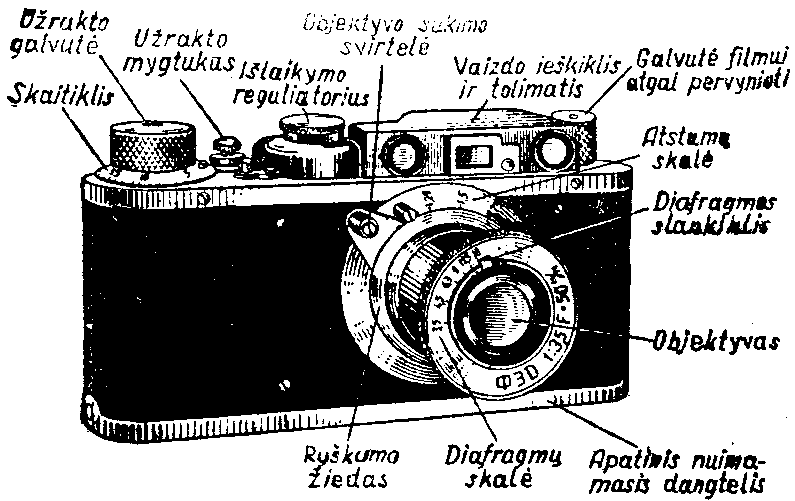
\includegraphics[width=0.8\textwidth]{20-pav}
				\caption{Fotoaparatas FED}
				\label{fig:20}
			\end{figure}
			jis labai populiarus tarp tarybinių fotografų mėgėjų.

			Bendrieji konstrukciniai duomenys aprašyti aukščiau. Savitos ypatybės yra tokios.

			FED --- lengviausias, mažiausias ir portatyvus aparatas. Jo korpuso forma yra patogi, su apvaliais galais. Įdedant filmą, nuimamas apatinis korpuso dangtelis.

			Objektyvas --- paskaidrintas keturių lęšių anastigmatas FED (``Industar 10''), kurio šviesos stiprumas --- 3,5, o židinio nuotolis --- 5 \textit{cm}; objektyvas įstatytas įstumiamame įtvare. Jo atstumų skalės padalos tokios (nestandartinės): 3,5 --- 4,5 --- 6,3 --- 9 --- 12,5 --- 18. Keičiamieji objektyvai įsukami į korpuso žiedą.

			Ryškumas nustatomas, sukant už svirtelės objektyvą. Ryškumas ir kadro ribos nustatomi vienas paskui kitą, žiūrint pro atskirus tolimačio ir vaizdo ieškiklio langelius.

			Šilkinė gumuota užrakto užuolaidėlė juda iš dešinės į kairę palei kadro ilgį. Užraktas automatiškai atlieka septyneriopą išlaikymą (nestandartiškai): \nicefrac{1}{20}, \nicefrac{1}{30}, \nicefrac{1}{40}, \nicefrac{1}{60}, \nicefrac{1}{100}, \nicefrac{1}{200} ir \nicefrac{1}{500} sekundės. Išlaikymo reguliatorių galima nustatyti, tik prisukus užraktą.

			Mažiausias fotografavimo atstumas, kai nenaudojami papildomi optiniai prietaisai, --- vienas metras.

			Aparato dydis --- 133 \texttimes 55 \texttimes 30 \textit{mm}; svoris --- apie 500 \textit{g}.
		\subsection*{\textit{``Zorkij'' --- kinofilminis 24 \texttimes 36 mm aparatas}}
			Mažojo formato fotoaparato ``Zorkij'' kamera ir mechanizmas beveik tokie pat kaip ir aparato FED. Skiriasi tuo (neskaitant kelių detalių išvaizdos), kad korpusas tvirtesnis, automatinis išlaikymas tikslesnis, tolimatis koordinuojamas su keičiamaisiais objektyvais.

			Objektyvas --- paskaidrintas keturių lęšių anastigmatas ``Industar 22'', kurio šviesos stiprumas --- 3,5 ir židinio nuotolis --- 5 \textit{cm}. Įtvaras --- įstumiamas arba neįstumiamas. Diafragmų skalės padalos už pilnosios angos sutampa su standartine eilute: 3,5 --- 4 --- 5,6 --- 8 --- 11 --- 16.

			Mažiausias fotografavimo atstumas --- vienas metras.
		\subsection*{\textit{``Zorkij 3'' --- kinofilminis 24 \texttimes 36 mm aparatas}}
			Mažojo formato fotoaparatas ``Zorkij 3'' (21 pieš.) --- tai žymiai patobulintas aparato ``Zorkij'' modelis.

			Aparato ``Zorkij 3'' korpuso užpakalinė sienelė padaryta nuimama. Tai leidžia patogiai įdėti filmą į apartą arba išimti iš jo, valyti, tikrinti keičiamųjų objektyvų priderinimą (matiniu stiklu, priglaudžiamu prie kadrinio rėmelio), o taip pat atkirpti (tamsioje patalpoje) išfotografuotą filmo dalį ryškinimui.

			Objektyvas --- paskaidrintas šešių lęšių anastigmatas ``Jupiter 8'', kurio šviesos stiprumas labai didelis --- 2, o židinio nuotolis --- 5 \textit{cm}; objektyvas įtaisytas įstumiamame arba neįstumiamame įtvare.

			Tolimatis ir vaizdo ieškiklis turi bendrą okuliarą, dėl to kartu nustatomas ir ryškumas, ir kadro ribos.
			\begin{figure}[h]
				\centering
				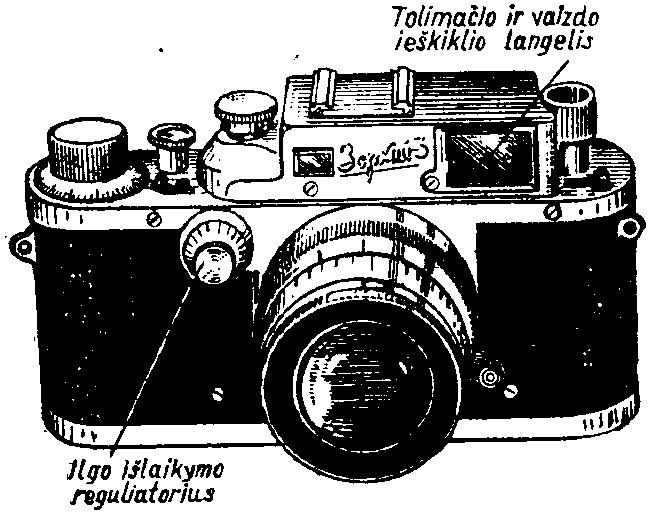
\includegraphics[width=0.8\textwidth]{21-pav}
				\caption{Fotoaparatas ``Zorkij 3''}
				\label{fig:21}
			\end{figure}
			Okuliaru galima padaryti optines pataisas ($\pm$ dioptrijos), kad toliaregiai ir trumparegiai fotografai galėtų fotografuoti be akinių.

			Prie užuolaidinio užrakto įtaisytas papildomas ilgo išlaikymo reguliatorius, kurio skridinys yra ant priekinės korpuso sienelės. Užraktas automatiškai atlieka dešimteriopą standartinį išlaikymą labai plačiame diapazone: 1 sekundė, \nicefrac{1}{2}, \nicefrac{1}{5}, \nicefrac{1}{10}, \nicefrac{1}{25}, \nicefrac{1}{50}, \nicefrac{1}{100}, \nicefrac{1}{250}, \nicefrac{1}{500} ir \nicefrac{1}{1000} sekundės. Yra padala \textit{\foreignlanguage{russian}{Д}} ilgam išlaikymui ``dviem paspaudimais''.

			Mažiausias fotografavimo atstumas --- vienas metras.

			``Zorkij 3'' tikrai vertas patyrusio fotografo mėgėjo dėmesio.
		\subsection*{\textit{``Kijev'' --- kinofilminis 24 \texttimes 36 mm aparatas}}
			Bendruosius konstrukcinius duomenis žr. 46 -- 48 puslapiuose. Savitos mažojo formato aparato ``Kijev'' (22 pieš.) ypatybės yra tokios.

			Korpusas, kurio galai su nuožambiais kampais, turi atlenkiamą atramą aparatui pastatyti tiesiog ant stalo arba kito horizontalaus paviršiaus. Nuimama užpakalinė korpuso sienelė leidžia lengvai įdėti filmą į apartą bei išimti iš jo, valyti aparatą, atkirpti (tamsioje patalpoje) eksponuotąją filmo dalį ryškinimui ir justuoti (derinti) keičiamuosius objektyvus, priglaudus prie kadrinio rėmelio matinį stiklą.
			\begin{figure}[h]
				\centering
				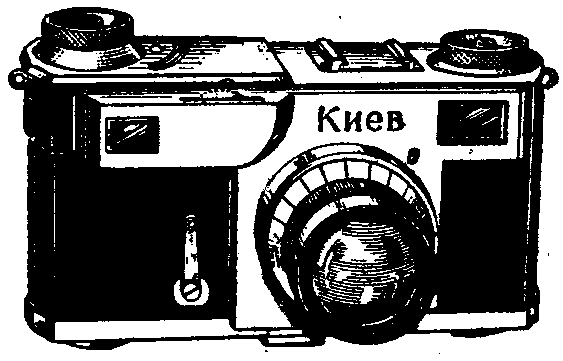
\includegraphics[width=0.8\textwidth]{22-pav}
				\caption{Fotoaparatas ``Kijev''}
				\label{fig:22}
			\end{figure}

			Objektyvas --- paskaidrintas šešių lęšių anastigmatas ``Jupiter 8'', kurio šviesos stiprumas labai didelis --- 2, o židinio nuotolis --- 5 \textit{cm} (įstumiamame arba neįstumiamame įtvare).

			Objektyvai ne įsukami, bet įtvirtinami korpuso žiede skląsteliu, dėl to jie pakeičiami greitai.

			Kai naudojamas pagrindinis objektyvas, ryškumas nustatomas, sukant patogų rievėtą ratuką, kyšantį korpuso viršuje. Nustatant ryškumą, nustatomos ir kadro ribos, nes tolimačio ir vaizdo ieškiklio okuliaras bendras. Pailginta tolimačio bazė\footnote{Atstumas tarp regėjimo ašių prietaiso plokštumoje.} (90 \textit{mm} vietoje 38 \textit{mm} FED tipo aparatuose) padidina ryškumo nustatymo tikslumą.

			Tvirta metalinė užrakto užuolaidėlė, judanti iš viršaus žemyn, palei kadro plotį, nesutrikdama veikia ir šaltyje. Užraktas automatiškai atlieka devyneriopą išlaikymą plačiame diapazone: \nicefrac{1}{2}, \nicefrac{1}{5}, \nicefrac{1}{10}, \nicefrac{1}{25}, \nicefrac{1}{50}, \nicefrac{1}{125}, \nicefrac{1}{250}, \nicefrac{1}{500} ir \nicefrac{1}{1250} sekundės. Išlaikymą galima nustatyti ir neprisukus užrakto, bet patariama pirma prisukti jį. Užraktas turi automatinį spaustuką pačiam fotografui nusifotografuoti; jis maždaug 9 -- 15 sekundžių uždelsia mechanizmo, automatiškai atliekančio išlaikymą, veikimą.

			Prisukamoji rankenėlė ne tik prisuka užraktą ir patraukia filmą, bet yra ir išlaikymo reguliatorius.

			Mažiausias fotografavimo atstumas --- 90 \textit{cm}.

			Aparato dydis --- 150 \texttimes 83,5 \texttimes 45 \textit{mm}; svoris --- 750 \textit{g}.
		\subsection*{\textit{``Kijev III'' --- kinofilminis 24 \texttimes 36 mm aparatas}}
			Mažojo formato fotoaparatas ``Kijev III'' (23 pieš.) skiriasi nuo aparato ``Kijev'' tuo, kad į jo konstrukciją įvestas fotoelektrinis eksponometras (prietaisas fotografavimo išlaikymui nustatyti, remiantis faktiniu objekto šviesumu).
			\begin{figure}[h]
				\centering
				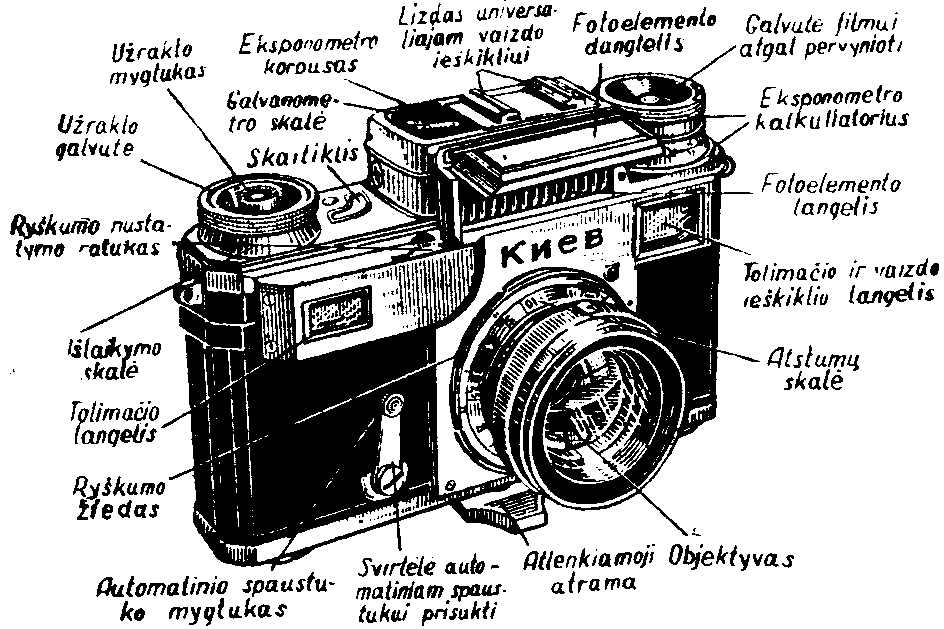
\includegraphics[width=0.8\textwidth]{23-pav}
				\caption{Fotoaparatas ``Kijev III''}
				\label{fig:23}
			\end{figure}
			Eksponometras sudarytas iš fotoelemento, galvanometro, varžymo ir mechaninio kalkuliatoriaus; jis sumontuotas aparato korpuso viršuje.

			Abu aparato ``Kijev'' modeliai yra tobuliausi fotoaparatai: patyrusiam fotografui jie teikia plačias fotografavimo galimybes.
		\subsection*{\textit{``Zenit'' --- kinofilminis 24 \texttimes 36 mm aparatas}}
			Mažojo formato fotoaparato ``Zenit'' (24 pieš.) konstrukcija panaši į aparato ``Zorkij''; korpusas aklinas; pagrindinis skirtumas --- kadro parinkimas ir ryškumo nustatymas, dėl kurių aparatas priskiriamas veidrodinių aparatų tipui.
			\begin{figure}[h]
				\centering
				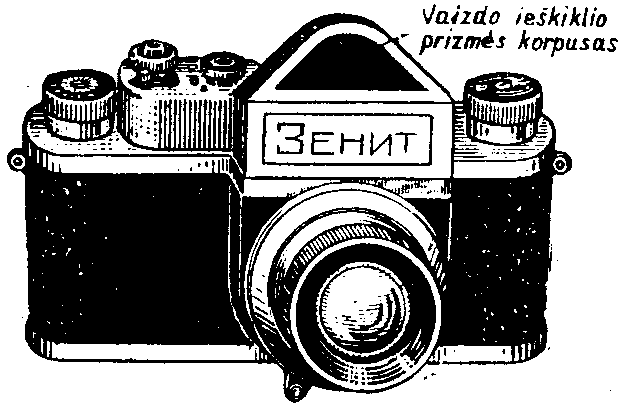
\includegraphics[width=0.8\textwidth]{24-pav}
				\caption{Fotoaparatas ``Zenit''}
				\label{fig:24}
			\end{figure}

			Objektyvas --- ``Industar 22'', kurio šviesos stiprumas --- 3,5, o židinio nuotolis --- 5 \textit{cm}. Užuolaidinis užraktas automatiškai atlieka penkeriopą išlaikymą: \nicefrac{1}{25}, \nicefrac{1}{50}, \nicefrac{1}{100}, \nicefrac{1}{250} ir \nicefrac{1}{500} sekundės.

			Vaizdo ieškojimo ir regimojo ryškumo nustatymo sistemą sudaro veidrodis, įtaisytas už objektyvo 45\degree kampu į optinę ašį, stiklas su matiniu paviršiumi, tiesioginio matymo prizmė (dukart apverčianti vaizdą) ir didinamieji lęšiai. Paspaudus užrakto mygtuką, veidrodis pakyla, atverdamas šviesos spinduliams kelią į fotografinį sluoksnį. Įdedant tarpinius žiedus, aparatas pritaikomas fotografuoti iš arti mažiems objektams, daryti reprodukcijoms.
		\subsection*{\textit{``Smena'' --- kinofilminis 24 \texttimes 36 mm aparatas}}
			Mažojo formato fotoaparatas ``Smena'' (25 pieš.), palyginus su jau aprašytomis kinofilminėmis fotokameromis, yra supaprastintos konstrukcijos, bet kai kuo yra ir pranašesnis. Jo korpusas iš plastmasės, užpakalinė sienelė nuimama. Objektyvas --- paskaidrintas trijų lęšių anastigmatas, kurio šviesos stiprumas --- 4,5, o židinio nuotolis --- 4 \textit{cm}. Diafragmų skalės padalos: 4,5 --- 5,6 --- 8 --- 11 --- 16 --- 22.

			Ryškumas nustatomas pagal atstumų skalę, sukant objektyvą. Vaizdo ieškiklis --- optinis.
			\begin{figure}[!h]
				\centering
				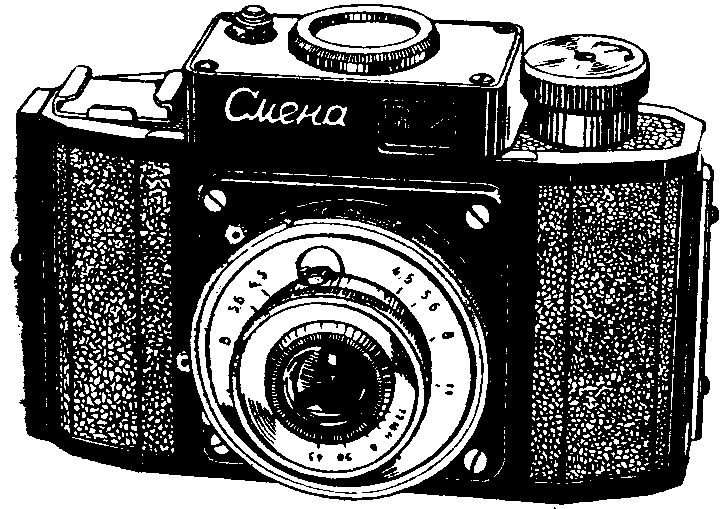
\includegraphics[width=0.8\textwidth]{25-pav}
				\caption{Fotoaparatas ``Smena''}
				\label{fig:25}
			\end{figure}

			Centrinis užraktas automatiškai atlieka penkeriopą išlaikymą: \nicefrac{1}{10}, \nicefrac{1}{25}, \nicefrac{1}{50}, \nicefrac{1}{100} ir \nicefrac{1}{200} sekundės.

			Filmas patraukiamas tiksliai per vieną kadrą; šis tikslumas išlaikomas mechaniniu būdu. Kadangi priimančiosios ritės vietoje būna standartinė uždara kasetė, pervynioti eksponuoto filmo atgal nereikia.

			Aparato dydis: 120 \texttimes 74 \texttimes 57 \textit{mm}; svoris --- 325 \textit{g}.

			Papildomieji objektyvai nenaudojami.

			Aparatas ``Smena'' skirtas gausiam fotografų mėgėjų būriui ir ypač jaunimui.
		\subsection*{KOKĮ FOTOAPARATĄ PASIRINKTI?}
			Šiuolaikinė fotografinių aparatų gamybos technika leidžia pasakyti: nėra blogų fotoaparatų --- yra blogų fotografų!

			Tačiau koks gi aparatas geriausias?

			Griežtai atsakyti į šį klausimą negalima. Iš tikrųjų, jeigu vienas kuris nors fotoaparatas būtų iš visų geriausias, tai visi kiti vargu ar bebūtų gaminami. O vis dėlto yra gaminami, perkami ir sėkmingai naudojami įvairių įvairiausi fotografiniai aparatai. Tai reiškia, kad kiekviena fotoaparatų rūšis turi kokių nors ypatingų savybių, kurios daro kaip tik šį tipą tinkamiausią tam tikrai paskirčiai. Sujungti visas gerąsias savybes ir pašalinti visus trūkumus viename fotoaparate neįmanoma; dėl to ir nėra tokio aparato, kuris tiktų visiems tikslams, kuris būtų vienodai patogus visais atžvilgiais. Tai, kas vienais atvejais yra trūkumas, kitais atvejais gali būti pranaši savybė, ir atvirkščiai. Pavyzdžiui, iš karto visos filmo juostos ryškinimas, nepatogus epizodiniam darbui, labai palengvina ekspedicijų fotografinių rezultatų apdirbimą. Nuimama mažojo formato kamerų (``Zorkij 3'', ``Kijev'', ``Smena'') užpakalinė sienelė teikia neabejotiną patogumą, bet kartu, nudengtas filmo dėjimo metu, vidinis aparato mechanizmas gali būti lengvai užterštas, ypač lauke, dulkingoje vietoje ir pučiant vėjui; galima sužaloti ir užrakto užuolaidėlę.

			Mūsų šalyje gaminamų masinių fotoaparatų suvestinę lentelę (4 lent.) skaitytojai ras 56 puslapyje.

			Plokštelė ar filmas? Didelis aparatas ar mažojo formato? Štai pagrindiniai klausimai, kylantieji kiekvienam, norinčiam pirmąkart įsigyti fotoaparatą. Tokiems skaitytojams padėti sudarėme 5 lentelę (žr. 57 psl.), kurioje palyginamos pagrindinės fotoaparatų rūšys.

			Pirmiausia reikia žinoti, ko iš būsimo fotoaparato norime.

			Plokštelinis fotoaparatas paprastas, jis pritaikytas įvairioms nuotraukoms daryti ir tinka daugumai atvejų, pasitaikančių fotografo mėgėjo praktikoje.

			Jeigu fotografas mėgėjas tik kartkartėmis darys po dvi tris nuotraukas, tai plokštelės jam patogesnės, nes dirbant su ritiniu filmu, ryškinimą tenka atidėti iki to laiko, kol bus eksponuota visa juosta su tuzinu (arba net su trimis tuzinais) nuotraukų. O jeigu reikės daryti 20 -- 30 nuotraukų vienoje vietoje, tai geresnis plačiafilmis aparatas.
\end{document}